% ------------------------------------------------------------------------

 \documentclass[11pt,twoside,a4paper]{report}
 \usepackage[latin1]{inputenc}
\usepackage{listings}
\usepackage[usenames,dvipsnames]{color}

 \definecolor{lightgray}{rgb}{0.95,0.95,0.95}
 \definecolor{darkred}{rgb}{0.8,0.2,0.2}
\lstset{ 
language=C++,
keywordstyle=\color{black}\bfseries,
stringstyle=\color{red},
commentstyle=\color{darkred},
basicstyle=\footnotesize,
numbers=none,
numberstyle=\footnotesize,
stepnumber=2,
numbersep=5pt,
%backgroundcolor=\color{white},
backgroundcolor=\color{lightgray},
showspaces=false,
showstringspaces=false,
showtabs=false,
frame=none,
tabsize=2,
captionpos=b,
breaklines=true,
breakatwhitespace=false,
escapeinside={\%*}{*)}
}





 \usepackage{amsmath}
 \usepackage{subfigure}
 \usepackage{placeins}
 \usepackage{caption2}
 \usepackage{floatflt}
 \usepackage{wrapfig}
 \usepackage[]{tocbibind}
 \usepackage{appendix}
 \usepackage{ifthen}
 \usepackage{times}                                          %true type fonts
 \pagestyle{headings}
 \usepackage[pdftex]{graphicx}                               %USE WHEN DOCUMENT IS PDFLATEX'ED!
 \usepackage[pdftex,plainpages=false,pagebackref]{hyperref}  %USE WHEN DOCUMENT IS PDFLATEX'ED! NO COLORLINKS
 \pdfcompresslevel=9                                         %USE WHEN DOCUMENT IS PDFLATEX'ED!
 \pdfoutput=1                                                %USE WHEN DOCUMENT IS PDFLATEX'ED!
 \hypersetup{
 bookmarksopen=true,
 bookmarksopenlevel=0,
 pdfauthor={Jochen Markert, Goethe-Universit�t, Frankfurt am Main},
 pdftitle={HYDRA manual},
 pdfkeywords={Hades, HYDRA, Magbolz, Heed}
}
\setcounter{tocdepth}{4}
\setcounter{secnumdepth}{4}

\newlength{\mylinewidth}
\setlength{\mylinewidth}{\linewidth}
\setlength{\textwidth}{159mm}
\setlength{\oddsidemargin}{0in}
\setlength{\evensidemargin}{0in}


\makeatletter
\newcommand\figcaption{\def\@captype{figure}\caption}
\newcommand\tabcaption{\def\@captype{table}\caption}
\makeatother

\newenvironment{narrow}[2]{
   \begin{list}{}{
      \setlength{\topsep}{0pt}
      \setlength{\leftmargin}{#1}
      \setlength{\rightmargin}{#2}
      \setlength{\listparindent}{\parindent}
      \setlength{\itemindent}{\parindent}
      \setlength{\parsep}{\parskip}}
\item[]}{\end{list}}

\newcommand{\goodgap}{
\hspace{\subfigtopskip}
\hspace{\subfigbottomskip}}

\renewcommand{\textfraction}{0.0003} % make large figures on page possible
%%% ------------------------------------------------------------------------
%%% ----------------------------------------------------------------------

%\hyphenation{}


\title{HYDRA2 manual} 
\author{Hades software group}
\date{\today} % Date


 \begin{document}


%NO NEED TO TYPE FILE EXTENSIONS IN \includegraphics:
 \DeclareGraphicsExtensions{.jpg,.pdf,.png}             %USE WHEN DOCUMENT IS PDFLATEX'ED!

% ------------------------------------------------------------------------
% Cover- Titelseite
\thispagestyle{empty}

\maketitle

\cleardoublepage
\thispagestyle{empty}


\pagenumbering{roman}

% ------------------------------------------------------------------------
 \cleardoublepage
 \tableofcontents
 %\cleardoublepage
 \listoffigures
 \listoftables

 \cleardoublepage

% ------------------------------------------------------------------------
 \pagenumbering{arabic}
 \setlength{\parskip}{1.0ex plus0.2ex minus0.2ex}             %set skip between paragraphs

 \clearpage
 \chapter{Software environment}


The HADES software environment HYDRA2 is base a C++ frame work based
on ROOT. The be able to compile and run HYDRA2 you therefore have to 
install ROOT and setup the .rootrc in your homedir.
The .rootrc is analyzed by ROOT at startup and can be used to setup
the default behaviour for ROOT. 

For HYDRA2 we set the path from where macros are started and the name
of the macro which should be loaded at startup to load the HYDRA2 libaries
into the ROOT session. The libries provide all functionalty of HYDRA2.
The most simple version of .rootrc is shown in listing \ref{rootrc}.


\lstinputlisting[label=rootrc,caption=.rootrc]{macros/.rootrc}



\section{Documentation}

Since HYDRA is build on top of ROOT using C++ the user should
learn ho to use C++ and ROOT. ROOT has a very rich documentation, 
tutorial and how-to section.


\begin{itemize}

\item C++ : http://www.cplusplus.com/
      \newline
       http://www.cppreference.com/wiki/

\item Fortran  :   http://www.star.le.ac.uk/~cgp/prof77.html

\item ROOT 
       \begin{itemize}
       \item classes :	http://root.cern.ch/drupal/content/reference-guide
       \item tutorials : http://root.cern.ch/root/html/tutorials/
       \item how-to : http://root.cern.ch/drupal/content/howtos
       \item manual : http://root.cern.ch/drupal/content/users-guide
       \end{itemize}
\item HYDRA 
  \begin{itemize}
    \item online documentation (classes) :  http://www-hades.gsi.de/docs/hydra/classDocumentation/
    \item code version: see \ref{Chapter_trac}
   \end{itemize}
\end{itemize}

\section{Software locations at GSI}\label{Chapter_softlocations}

HYDRA2 and the former HYDRA has been developed over many years. Operating
systems have been changed during that time. We decided to create the HADES
software tree in a common place which is accessible form all HADES machines 
and the batch farm. A branch for OS (debian) is added.
 

\begin{lstlisting}

binaries are installed here:
/misc/hadessoftware/etch32/install/hydra-dev
  
source code for compilation is here:
/misc/hadessoftware/etch32/hades/hydra-dev
  
\end{lstlisting}

hydra-dev indicates the development status of HYDRA2. If you use this version 
be aware that it can be recompiled and changed at any time! For DST production
and analysis we provide fixed release versions. Each install dir keeps a defalls.h
script to set the full environment for HYDRA2

\begin{lstlisting}

to set the HYDRA2 environment:
. /misc/hadessoftware/etch32/install/hydra-dev/defall.sh
  
\end{lstlisting}

The content of the defall.sh script is shown in \ref{defall}.
Inside the script the following environtment variables
are set:

\begin{enumerate}
 \item \verb+ROOTSYS    : The install location of ROOT+
 \item \verb+HADDIR     : The global HYDRA2 install location+
 \item \verb+MYHADDIR   : The user   HYDRA2 install location (optional)+
 \item \verb+CERN_ROOT  : The install location for the CERNLIB+
 \item \verb+ORACLEHOME : The install location of ORACLE+
 \item \verb+ORA_USER   : The HADES ORACLE user to access parameters+
\end{enumerate}


The \verb+MYHADDIR+ is needed if a local changed HYDRA library should be 
loaded/linked with HYDRA libs form the global HYDRA dir (\verb+HADDIR\lib+). 
This allows the user to have a local dir where changes can be applied. The 
seach order for the the linker/compiler takes the local libdir (\verb+MYHADDIR\lib+)
first and second the global dir. The ORACEL variables have to be set if
HYDRA2 should be compiled with ORACLE access (switch in Makefile).
\verb+CERN_ROOT+ specifies tyhe CERNLIB location. The CERNLIB is needed
for the GEANT simulation of HADES.

\clearpage

\lstinputlisting[label=defall,caption=defall.sh]{macros/defall.sh}

\clearpage


\section{How-to install}

\subsection{HYDRA2}

HYDRA2 cand be run and installed in ether 32bit or 64bit
version. A tarball including ROOT, CERNLIB, GARFIELD and gsl
sources is located in

\begin{lstlisting}
/misc/hadessoftware/squeeze64/packages/hades_packages.tar.gz
\end{lstlisting}

This tar contains installHades.sh which does the full 
installation of the software tree. The ORACLE client software
has to installed before. The needed package you will find
on the ORACLE webpage (see chapter \ref{Chapter_ORA_install}).

All other instructions of the setup are documented inside the
the tar file. For HYDRA2 you can ignore the dicussion of
32bit/64bit.



\subsection{HYDRA}

The instruction below assume 32bit system. Currently
we compile our software 32bit. On the batchfarm we run in
64bit systems using the compatibility libs from Debian.
To compile everything in native 64bit is not easily possible
because of the CERNLIB. You can try yourself, but you will
get no support from GSI. For future we have to find a way
to get rid of the old CERNLIB.

\subsubsection{CERNLIB installation at GSI}\label{Chapter_CERNLIB_install}

The CERNLIB is needed for the \verb+HGeant+ detector simulation of HYDRA2.
Currently Cernlib 2006 is used with g77 compiled 32bit. The 
installation is not straight forward and needs special patches.
For our current system Debian etch32 you can install the CERNLIB
in the following way:

\begin{lstlisting}
 
  find the script:
 /misc/hadessoftware/etch32/install/installCernlib.sh
 
 edit the script to set you fortran compiler (g77 recommended)
 
 run the script
 
\end{lstlisting}

\subsubsection{ROOT installation at GSI}\label{Chapter_ROOT_install}

Our current installation of ROOT is using a private 
gsl (Gnu Scientificc Library). Therfore the first step is to install gsl:

\begin{lstlisting}
#-------------------------------------------
#Install gsl

tar -zxf  gsl-1.12.tar.gz
mv  gsl-1.12  gsl-1.12_make
cd gsl-1.12_make

./configure  --prefix=/misc/hadessoftware/etch32/install/gsl-1.12
make -s -j16

# run test suite (optional)
make check > log_test.txt 2>&1
make install
#-------------------------------------------
\end{lstlisting}



HYDRA2 currently is using ROOT 5.22.00a and soon will be update to 5.28.00.
The GSI configuration for compiling ROOT is listed below.

The location at GSI: \verb+/misc/hadessoftware/etch32/install/root-5.22.00a+

\begin{lstlisting}

cd  /misc/hadessoftware/etch32/install

svn co https://root.cern.ch/svn/root/tags/v5-22-00a root-5.22.00a

cd  root-5.22.00a

export ROOTSYS=`pwd`

 ./configure linux --enable-exceptions \
                        --enable-soversion \
                        --enable-table \
                        --enable-asimage \
                        --enable-opengl \
                        --enable-minuit2 \
                        --enable-mathmore \
                        --enable-roofit \
                        --enable-xml \
                        --disable-mysql \
                        --disable-globus \
                        --disable-explicitlink \
                        --disable-rpath \
                        --disable-pythia6 \
 			--with-gsl-incdir=/misc/hadessoftware/etch32/install/gsl-1.12/include \
 			--with-gsl-libdir=/misc/hadessoftware/etch32/install/gsl-1.12/lib

make

#-------------------------------------------
\end{lstlisting}

\subsection{ORACLE client installation}\label{Chapter_ORA_install}

Currently we use at GSI ORACLE 10.2.0.1client to access the data base.
If you want to use data base support for HYDRA2 you have to install
The ORACLE software at your local system. The packages can be downloaded
from
\newline
http://www.oracle.com/technetwork/database/enterprise-edition/downloads/index.html

Follow the instructions.



\begin{lstlisting}[language=bash]
---------------------------------------------------------------------------------
# checkout a repository

# get full repository from trunk (main branch) into a folder hydraTrans
svn co https://subversion.gsi.de/hades/hydraTrans/trunk /mypath/hydraTrans

cd /mypath/hydraTrans

cp /misc/hadessoftware/etch32/admin/hsc-dev defall.sh

edit the path to ROOTSYS and HADDIR according to your installation

cp admin/*.mk .
cp admin/Makefile .

edit the Makefile according to your needs:
INSTALL_DIR      = /mypath/hydraTrans
USES_RFIO        = no

. ./defall.sh
make -s -j16

make install
---------------------------------------------------------------------------------
\end{lstlisting}

\subsubsection{HGeant}

\begin{lstlisting}
   1. Install Root, Cernlib and Hydra.
   2. Setup your shell environment (including Root,Cernlib and Hydra settings)
   3. Create a source code directory:
          
          mkdir /mypath/hgeant-version (use appropriate version number or snapshot date)
   
   4. Checkout the HGeant code:
      HGeant code is located in CVS: CVSROOT=/misc/halo/repos/simul
          cd /mypath/hgeant-version
          /misc/hadessoftware/etch32/admin/full-hgeant-checkout.sh CVSROOT 
   
   5. Build it:
          cp /mypath/hgeant-version/admin/Makefile /mypath/hgeant-version/
          edit INSTALL_DIR
          
          make
   6. Install it:
          make install
   7. Remove the files created durning build:
          make distclean
\end{lstlisting}

\section{HYDRA2 source code repositories at GSI}\label{Chapter_HYDRA_repos}

The Hades Subversion (svn , http://subversion.tigris.org/) repositories are 
located at the GSI web-server. Some information about subversion at GSI can 
be found at http://wiki.gsi.de/Linux/SubVersion The access authentification 
uses the ORACLE data base of GSI. Read permission is granted anonymously. For 
commiting code you have to have an account at http://www-oracle.gsi.de/ . 
This is the same account as used for the documentation of working time or 
the radiation savety. You do not need to have GSI linux or windows account 
to get an user account. The user name has to added to the subversion access 
management. Mail your user name and which directories you want to work with 
to j.markert@gsi.de.


For the documentaion of subversion see http://svnbook.red-bean.com/

\begin{lstlisting}
---------------------------------------------------------------------------------
# checkout a repository

# get full repository from trunk (main branch) into a folder hydraTrans
svn co https://subversion.gsi.de/hades/hydraTrans/trunk hydraTrans

# get a directory from the repository trunk (main branch) into a folder hydraTrans
svn co https://subversion.gsi.de/hades/hydraTrans/trunk/mdc hydraTrans/mdc
---------------------------------------------------------------------------------
# view all commands
svn help

# view help on commands
svn help status 
---------------------------------------------------------------------------------
# most usefull commands
# to work on the local working copy

[file] means filename is optional. In this case the commands
apply to all files in the current directory

// show local changes (stat=status)
svn stat    [file]                                        

// show local changes and changes on the server (-u == in update mode)
svn stat -u [file]                                        

// show modification of a file against a revision
svn diff [file]                                           

// schedule a new file for adding. Needs commit afterwards to 
// send it to the repository
svn add file                            

// update file to newest revision
svn update [file]                                         

// send file [or all modified files] to repository (requires access 
// permissions). takes the user name from checkout log
svn commit -m "your comment" [file]                       

// send file [or all modified files] as agiven svn user to repository 
// (requires access permissions). helpful to commit from a checkout 
// dir of another user
svn --username yourname commit -m "your comment" [file]   
                                                          
                                                          
                                                          


// show graphical diff of file to svn base revision
tkdiff file                                               
// show graphical diff of file to newest svn head revision
tkdiff file -r head                   

\end{lstlisting}




\subsection{Web-frontend TRAC} \label{Chapter_trac}

The GSI IT provides Trac , a web-frontend for the subversion repositories, 
running on the apache webserver. This web-frontend replaces our old CVS frontend. 
Besides the standard source browsing features Trac support a bug tracking 
system (see below).

https://subversion.gsi.de/trac/hydra

https://subversion.gsi.de/trac/hydraTrans

Up to now the bugs of Hydra have been reported in the Hades Forum. Since our new web frontend for subversion supports a simple bug tracking system I will use this feauture.

The bug tracking systen has the following features:

\begin{enumerate}
    \item Each registered user of the HADES repositories (see ORACLE account above) can add new bug reports. In Trac the reports are called "tickets". You have to login to Trac to add a new Ticket.
    \item The ticket can contain code snippets and it is possible to attach pictures
    \item Each ticket can be accepted and assigned to a person who should take care about it.
    \item The ticket also can be reassigned to another person.
    \item The tickets are uniquely numbered like \verb+"#1"+.
    \item If a bug is fixed. The developer will quote the bug number in the commit comment. Trac will recognize the bug number \verb+#number+ and create a link to the bug report.
    \item After fixing the bug. The ticket can be set to status fixed and will be removed from the list of active bugs. All bugs can be still displayed.
    \item Any change on the bug report will cause a mail to the assigned person and the person who created the report.
\end{enumerate}






 \clearpage
 \chapter{The analysis framework}


\section{The HADES class}

The \verb+Hades+ class is the fundamental class which controls and 
coordinates all the different parts of the reconstruction 
software. Essentially it is formed by %see figure [*]):

%Figure: Hades class structure.
\begin{enumerate}
    \item a data source where to read event data from.
    \item a \verb+HTaskSet+ storing the tasks to be performed for each event.
    \item a \verb+HEvent+ where to store the event in process.
    \item a \verb+HSpectrometer+ created during initialization and 
          storing information.about the spectrometer's structure.
    \item a database where to read reconstruction parameters from.
    \item a \verb+ROOT+ output tree.
    \item an output file. 
\end{enumerate}

There must be one and only one object instantiating the Hades 
class for a execution of the program, that is, the \verb+Hades+ class 
is a \verb+soliton+. This object is accessible from every part of 
the program through a global pointer which is called \verb+gHades+. 
For more information on this class and the services provided by 
it, check the reference documentation.

\section{Classes to contain data}

\subsection{The event structure}

An event is the record of all physical interactions in the detector 
resulting from the reaction between a beam particle and the target, 
and it can be real or simulated. A calibration event contains the 
response of one or several detectors to one or several particles or 
to a calibration signal (a laser signal, for example). The event is 
the unit for the data processing. From the reconstruction program's 
point of view, an event is an object instantiating some \verb+HEvent+ 
subclass and holding all relevant information coming from a 
beam-target interaction or resulting from a calibration signal. The 
event can contain both the original data coming from the spectrometer 
(raw data) and the more elaborated data which result from the 
reconstruction process.

One event is reconstructed in steps, so each step in the reconstruction 
process produces one level of reconstructed data. The number and kinds 
of reconstruction levels (or data levels) which are stored in an event 
is not fixed beforehand, since it can change as a function of the kind 
of event (simulated or real), as well as the specific task we want to 
accomplish at a given moment. If, for example, we are studying the 
calibration for the MDC we are not required to bother with the data 
level of the other detectors, or even with those MDC levels which are 
not used at that moment.
There is only one \verb+HEvent+ object within the \verb+Hades+ soliton. 
This \verb+HEvent+ object acts as a central repository, globally 
accessible, with all the information for one event, storing also 
structural information about that event. In this way, the different 
components of the reconstruction program (event display, data input, 
reconstruction algorithms, etc.) can access the event information in 
an independent way.

Data contained in an event are \verb+HDataObject+ objects. Within each 
event, these objects are organized in categories, that is, the event 
holds ``categories'' and these categories hold the data objects. 
During the initialization of the program the user decides which 
categories (how many and what kind of) he wants to have in the event, 
as well as the kind of data objects stored in each category.
To access a particular category within an event, one can use the 
\verb+getCategory(Cat_t aCat)+ function from \verb+HEvent+. This 
function returns the event's category identified by ``aCat'', 
where ``aCat'' is the value of a constant which univocally identifies 
one particular category (for example, \verb+catMdcRaw+ for the 
category holding raw data in the MDC).
As for the event storage in an output file, ROOT provides us with 
an automatic mechanism to store any ROOT object into a file, this 
can seem enough at a first glance. However, it turns out to be 
convenient to store the event's information in a more adequate and 
ordered form for its further analysis. In particular, we want to 
store event information using a ROOT tree. This is the reason for 
the function \verb+makeBranch()+ in the \verb+HEvent+ 
declaration \footnote{ In principle, ROOT has an automatic mechanism 
to build a tree from any object, however this mechanism doesn't provide 
the flexibility required for an object as complex as HEvent}.
In addition to storing the data objects we must be able to clear the 
information held in a \verb+HEvent+ so as to leave free place for 
the next event. This can be better understood watching the basic 
reconstruction cycle. The steps are the following:

\begin{enumerate}
\item Clear information in the current event; 
\item Read information from the active data source; 
\item Launch the reconstruction for the current event; 
\item Store the event data in an output file. 
\end{enumerate}

To accomplish the first step in this list we can use the functions 
\verb+Clear()+ and \newline \verb+clearAll(Int_t level)+. The first of them 
clears all data objects in the event but preserves its structure. 
The second one, on the other side, deletes both the data objects 
and the part of the event's structure which is selected by the 
parameter ``level'' \footnote{ For example, if level=0 every 
data object, as well as the whole event structure will be deleted, 
otherwise, if level>0, only cleared.}.
These are the fundamental characteristics of a general event. Now 
we will see different kinds of event and how the previous functions 
are implemented for each of them. 

%If you prefer to know more about the ``categories'' before, just jump to section [*].

\subsubsection{The partial event: HPartialEvent}

As its name suggests, a partial event is part of an event under 
reconstruction. In fact it is each part of an \verb+HRecEvent+ which 
has to do with a particular detection system. So, for Hades, we 
have one partial event for the RICH, another one for the MDC, etc.
Each partial event holds an array with all the categories belonging 
to it; so we can get any of them through the \verb+getCategory()+ method.
Beside the categories, each partial event maintains a ``reconstruction level'' 
in the same way as \verb+HRecEvent+. This allows one to know what is the 
state of the reconstruction for some event.
Obviously, this kind of event has also all the functions required to 
any ``HEvent'', like those intended to build an output ROOT tree 
starting from the array of categories held by the event.

\subsubsection{The simulated event}

The simulated events are the events produced by the Hades simulation 
program \verb+HGeant+. Simulated events can be used as input for the 
reconstruction program instead of real ones, therefore the simulated 
events must have the same structure as the real ones, so that the 
software can seamlessly process both real and simulated events. As 
for now this is achieved by using the same class both for simulated 
events and events under reconstruction.
The extra information in a simulated event, regarding kinematics, 
is stored in a dedicated partial event within the event under 
reconstruction.



\subsection{The data container}

A category is essentially a container of objects within an event, with 
the extra point that every object in a category belongs to (instantiates) 
the same class. For example, the raw data for MDC make up a category, 
but raw data in the RICH correspond to a different category since they 
are instances of a different class. Other categories can be the one 
storing calibrated MDC data, hits, tracks, particle candidates, etc.

The category concept is represented by the \verb+HCategory+ class. In 
fact this is an abstract class which declares a basic API to be implemented 
by any kind of category. These implementations correspond to different 
strategies for storing data, both in memory and in file(s). 

%In figure [*] you can see the HCategory's definition, as well as some inherited classes.

%Figure: HCategory structure

A category's API must have functions to access the data objects held by it. 
This access can be of two kinds: 
\begin{enumerate}
\item one can ask for one single data object or a set of them verifying some condition, 
\item one can iterate on all or part of the objects held by a category. The first mode requires random access, the second mode needs sequential access only.
\end{enumerate}

To access a particular object in a category we need ``something'' which 
identifies it in a univocal way. This ``something'' is an object instantiating 
the \verb+HLocation+ class and it's nothing more than an array of indexes. 
So, as we can see, it's as if data objects in a category were stored in a 
multi-dimensional matrix. Summarizing, each object is stored in a category 
at the location defined by a set of indexes encapsulated in a \verb+HLocation+ 
object; to access the data object we can use \verb+getLocation(HLocation &loc)+. 
The following example will help to make it clearer:

\begin{lstlisting}

{
  // Let's say, cat is a category with raw MDC data.
  HCategory *cat;
  // A raw hit in an MDC
  HMdcRaw *raw;
  // A new location object
  HLocation loc;

  // Let's set loc pointing to the fourth hit at the first layer 
  // of MDC 2 in the second sector. For this, we need to call
  // HLocation::set(n,...) with the number of indexes in the
  // location as the first argument, and then the actual indexes
  // themselves, in order:
  loc.set(4,1,1,0,3);     // all indexes start at 0!

  // Let's set raw pointing to the desired data object. This is
  // accomplished by calling the getObject(loc) method from
  // class HCategory. This method returns a pointer to the
  // object in the category at the location given by the
  // method's argument (loc).
  raw=cat->getObject(loc);
}
\end{lstlisting}


If we want a set of data verifying some condition, then we can use 
\newline 
\verb+query(TCollection *aCol, HLocation &loc, HFilter &filter))+. 
This function places within the collection aCol every object in 
the category which verifies the condition given by the filter 
``filter'' \footnote{See the HFilter class in the reference 
documentation} and corresponding to the location ``loc''. If ``loc'' 
is omitted, then any location is valid. If ``filter'' is not 
specified every object corresponding to the location ``loc'' is 
added to the collection. Let's see an example:

\begin{lstlisting}
{
  // Let cat be a category with MDC raw data. Each raw data is 
  // identified by 4 indexes: sector, module, layer and cell.
  HCategory *cat;
  // Let array be the target array of selected data objects
  TObjArray *array;

  // Let's set loc pointing to the first module in the first sector
  HLocation loc;
  loc.set(2,0,0); //Again, indexes start at 0!

  // Let filter be a filter implementing condition ``cond1''
  HCond1Filter filter;

  // Do the job. Now we have array filled with those data 
  // objects in the category which correspond to the first 
  // module in the first sector of the MDC and verify the 
  // condition ``cond1''
  cat->query(array,loc,filter);
}
\end{lstlisting}

At the end we treat the iteration on all or part of a category. This 
is accomplished using iterators, in the Standard Template Library 
(STL) way. To get an iterator for a category we can use the function 
\verb+MakeIterator()+; this function will return an \verb+HIterator+ 
object iterating on the whole category. If we want to restrict the 
iteration to a location we can use the \verb+gotoLocation(HLocation &loc)+ 
method from \verb+HIterator+. Let's see now an example with an iterator 
running on all raw data for chambers 1 and 2:

\begin{lstlisting}

{
  // The usual stuff
  HCategory *cat;
  HMdcRaw *raw;
  HLocation loc;

  // Set loc pointing to sector 1, module 2
  loc.set(2,0,1)    // Remember, indexes start at 0!

  // Build the iterator up
  HIterator *iterator=cat->MakeIterator();

  // Now we do a loop on the data objects using the iterator we
  // got before. This is accomplished with a "while" loop whose
  // condition equals the pointer "raw" to the next data object
  // in the category and checks if "raw" is different from NULL.
  // Once raw==NULL the iteration stops.
  while ( (raw=(HMdcRaw *)iterator->Next())!=NULL) {
    raw->Dump(); //print the data object pointed to by "raw" 
  }
}
\end{lstlisting}

Besides having objects stored in a category we must be able to add 
new objects to that category. The adopted solution consists in the 
user having to ask the category for a place in memory (a slot) where 
to place the new object. Then the user instantiates the object using 
the ``new with placement'' \footnote{The ``new with placement'' 
operator is used to instantiate an object at a predefined memory 
address. The syntax to instantiate an object of class, let's say 
HMdcRaw, at the address pointed at by a pointer named ``pMemAddress'' 
is: ``raw=new(pMemAddress) HMdcRaw'', where, ``raw'' is a pointer 
to HMdcRaw. Note that the ``new'' operator does not need to actually 
allocate memory but uses the memory pointed at by ``pMemAddress'', 
assuming it is already allocated} operator. In case the object is not 
instantiated using the ``new'' operator, what we have is just a piece 
of memory, not a real object. That means, for example that the virtual 
table is not built and therefore no virtual function can be called. 
Since each object in a category is associated with a location, to get 
a slot we use the method \verb+getSlot(HLocation &loc)+ if we know all 
indexes of the location, or we can use \verb+getNewSlot(HLocation &loc)+ 
if we know the indexes of the desired location, except the last one. 
Any of these two functions will return a pointer to the requested slot, 
or NULL if no slot was available at that location.

To summarize:
\verb+getObject(HLocation &loc)+ returns a pointer to the object at 
location loc, or NULL if that object does not (yet) exist.
\verb+getSlot(HLocation &loc)+ returns a pointer to (free) memory 
where a new object, corresponding to location loc in the category, 
can be instantiated, i.e. a pointer to slot loc.
\verb+getNewSlot(HLocation &loc)+ returns a pointer to the next free 
memory slot of the category following location loc, where a new object 
can be instantiated.

The main reason to let the category do the memory management instead of 
simply using the C++ ``new'' operator comes from the large number of 
data objects instantiated per event, and the large number of events 
to process. The ``new'' operator calls a costly routine in the operating 
system to get the requested memory. However a category can have a 
preallocated block of memory for the data objects which are going to be 
instantiated; this can speed up memory management because the category 
knows beforehand the size of the data objects which are going to be 
instantiated, as well as the kind of memory request it will be asked 
for. Let's now see an example:

\begin{lstlisting}

{
   //The usual stuff
   HLocation loc;
   HMdcRaw *raw;
   HCategory *cat;
   ...
   // Set loc pointing to sector 2, module 2, layer 1, cell 1
   loc.set(4,1,1,0,0)   // indexes start at..., well, you know it!
   // Ask for a slot
   raw=cat->getSlot(loc);

   // If the slot is valid (raw!=NULL), instantiate the object
   if (raw!=NULL) raw=new(raw) HMdcRaw;
   else Error("No slot available");
}
\end{lstlisting}

Below follows the description of the variuos kind of categories which 
have been implemented. This description deals with specific issues for 
each category, in particular their implementation.

\subsubsection{The HMatrixCategory}

This kind of category stores data objects in a matrix-like structure. 
In this way, when we ask for an object in the category, the location 
indexes which identify the objects are the same as the indexes of the 
underlying matrix. To initialize a matrix category one needs to provide 
the following data to the constructor:
\begin{enumerate}
    \item Number of indexes in the matrix;
    \item Maximum value for each of the indexes (that is, the matrix dimensions);
    \item fillRate; this is a number between 0 and 1 which corresponds to the maximum fraction of occupied locations we expect. 
\end{enumerate}

Looking in more detail into this category's implementation we notice that 
the mentioned matrix is actually linearized, i.e. in practice, the data 
objects are stored in a linear array (a \verb+TClonesArray+ from ROOT).
The internal structure of the category is the following: on one side we 
have a \verb+TClonesArray+ A with every data object, and we have an 
\verb+HIndexTable+ object T which behaves as a matrix of integers. When 
we are looking for an object associated with a location, we fetch from 
table T the matrix element corresponding to the indexes of that location. 
This matrix element is an integer giving in turn the position of the 
requested data object in the array A.

In this way it is not necessary to reserve for A all the memory which 
would be used if every location were filled and we can keep the 
\verb+TClonesArray+ without holes (this fact is important when we want 
to store the array in an output file). We have already said that 
\verb+HIndexTable+ behaves as an integer matrix. However, again, we can 
see that internally we have a linear array of integers. This is done to 
be able to work with an arbitrary number of indexes. 

\subsubsection{The HCategorySplit}\label{Chapter_catsplit}

To understand what this category does, we have to define beforehand the 
idea of ``terminal'' which will be used in the remaining of this section. 
Given a category where each data object is identified by a location of n 
indexes, we call ``terminal'' the location with n-1 indexes. An example 
will make this clearer: let's consider raw data in the MDC. Each data 
object is identified by 4 indexes (sector, module, layer, cell), therefore 
a ``terminal'' corresponds to a layer (location with 4-1=3 indexes).
What makes a \verb+HCategorySplit+ special is its ability to store the 
data objects for each ``terminal'' in an independent \verb+TClonesArray+, 
so that when generating the ROOT output tree we have one branch for 
each ``terminal''.
The category is internally made up of a matrix of pointers to 
\verb+TClonesArray+ objects. These, on their side, hold the data objects 
for each ``terminal''. As usual, the mentioned pointer matrix is realized 
in practice as an array. 

%You can see this structure in figure [*]
%Figure: HCategorySplit structure

Using \verb+TClonesArrays+ directly brings about an important consequence: 
one should not leave holes on the nth index when filling a \verb+HCategorySplit+. 
If this rule is not respected one will get a ``segmentation violation'' 
when storing the category in split mode. This means we will not be able to 
write to a file in split mode if we have one object at (1,2,1,0) and another 
at (1,2,1,2) and nothing in (1,2,1,1). But there is no problem having one in 
(1,2,1,0) and another at (1,2,3,0), or if we store data in non split mode.
As for initialization, this is done in two steps: In the first step, when the 
category is instantiated, one must set:
\begin{enumerate}
    \item Class name for the data objects to be stored in the category;
    \item Number of indexes needed to identify one ``terminal'';
    \item Dimensions of the ``terminal'' matrix;
    \item Pattern to name each of the branches for the different ``terminals''. In order to produce those names, a loop is done on all the active ``terminals'' in the category and for each ``terminal'', its location is matched against the before-mentioned pattern in order to produce a unique name. The matching is done by copying each character in the pattern to the branch's name until a sequence like ``%i%'' is found, which is substituted by the value + 1 of the i-th index in the location for the current ``terminal'', then the following characters in the pattern are copied to the branch's name until another sequence like ``%i%'' is found and so on until one reaches the end of the pattern. For example, if our category has 3 indexes and the ``terminal'' matrix has dimensions 2*2; a pattern like ``S%0%.M%1%'' will cause the branches to be created with names:
     \begin{itemize}
       \item S1.M1
       \item S1.M2
       \item S2.M1
       \item S2.M2
     \end{itemize} 
\end{enumerate}
The second step consists in calling one of the \verb+setup()+ functions to 
set the active ``terminals'', that is which modules we want memory and an 
output branch for. In order to set this, two ways are foreseen: 
\begin{enumerate}
 \item by providing the number of active ``terminals'' and their id numbers, or 
 \item by providing a table of integers (one per module) where a -1 stands for an inactive ``terminal'' and a number greater than 0 corresponds to the number of data objects expected for that ``terminal''. 
\end{enumerate}

\subsubsection{The HCategoryMatrixSplit}

Essentially it is the same as the \verb+HCategorySplit+, in fact, it inherits 
from \verb+HCategorySplit+. The main difference between the two is that 
\verb+HCategoryMatrixSplit+ uses \verb+HClonesTable+ objects instead of the 
\verb+TClonesArrays+. A \verb+HClonesTable+ is a descendant of \verb+TClonesArray+, 
but modified in order to allow for having holes even in split mode. On the other 
hand it is more complex and slower when accessing one particular data object.

\subsubsection{The HLinearCategory}

This is the simplest kind of category, in fact, an \verb+HLinearCategory+ is 
nothing more than a wrapper to a \verb+TClonesArray+, so the latter can be 
used within the Hydra framework. Therefore, the data stored in a \verb+HLinearCategory+ 
are identified by one single index (the location has just one index) which 
corresponds to the position of the data object in the underlying \verb+TClonesArray+.
This category can be useful in a variety of situations where data are accessed 
sequentially only, e.g. for calibration. Indeed, if we want to go from raw data 
in the Mdc to calibrated data, each raw datum is identified by four indexes 
(sector, module, layer, cell). The first step is to read from the acquisition 
system and place the data into the ``catMdcRaw'' category. After that the data 
are calibrated sequentially. In this example, one possibility is to place the 
data in the category without an order (putting data in a \verb+HLinearCategory+ 
as we read them) and store the four indexes as a data member of the data object. 
Later, during calibration, we iterate over all data objects, and for each of 
them we do the calibration with the parameters specified by the indexes stored 
in the data object.

\section{Classes to manage the input/output of data}

This sections describes essentially which mechanisms are foreseen in the framework, 
both for data reading and writing. In the first case, the adopted solution must be 
able to deal with several input sources and, on the other hand, data output is always 
realized through ROOT files and using essentially, but not only, ROOT trees.

\subsection{Data input}

In this section we will describe how the data are read from the different available 
data sources. The only thing the Hades class needs to know is the definition of a 
``data source'' in terms of C++, that is, which methods are provided by a ``data source'' 
and their meaning. In this way we can call those methods without knowing which concrete 
source is used.
The abstract class defining a data source is \verb+HDataSource+, and mainly defines one 
function \verb+getNextEvent()+ which must be implemented by all the inherited classes. 
When this function is called, one event is read from the data source into the event 
structure. The returned value of the operation can be one of the following:

\begin{itemize}
    \item \verb+kDsOk+: the event was successfully read; 
    \item \verb+kDsEndFile+: we have reached the end of a file (set of data with the same reconstruction parameters), but more data are available; 
    \item \verb+kDsEndData+: we have reached the end of the data source; 
    \item \verb+kDsError+: error. 
\end{itemize}

Up to now there is provision made for two data sources within the Hades soliton. 
We can combine data sources, e.g. mix real with simulated data like it is used in the 
event embedding.
Another very important function of the \verb+HDataSource+ class is the \verb+init()+ 
method used during initialization. Within this method each particular data source 
must check whether an event object exists or not and if it doesn't exist then it 
is the data source's first responsibility to instantiate an event object. Usually, 
the data source will also have to add to the instantiated event object those 
categories where data will be read into. Note that if an event object or the 
needed categories do already exist, then the data source must not destroy them, 
but use them directly. 

\subsubsection{Data input from the Data Acquisition System: HldSource}

\verb+HldSource+ is the base class for those data sources reading data from the 
HADES data acquisition system (DAQ), either from file (in hld format) or from the 
event server (via TCP/IP). 
%The class structure can be seen in figure [*].
%Figure: HLdSource

The \verb+HldSource+ reads raw data in the order and format provided by the DAQ and 
puts them at their place within the event structure; this usually implies some reordering. 
This process is what is known as unpacking and is realized by unpackers (objects 
instantiating the \verb+HldUnpack+ class) within an \verb+HldSource+.

\verb+HldUnpack+ is an abstract class from which several different unpackers are derived, 
as \newline
\verb+HRichUnpacker+ or \verb+HTofUnpacker+. In fact, we have one different unpacker for 
each detection system in HADES (MDC, TOF, RICH, SHOWER, START), so each unpacker only knows 
how to deal with a particular kind of data, i.e. subevent(s). The most important method of 
this class is the \verb+execute()+ function, in which the unpacking process is realized. 
Another important function is \verb+init()+ which is used during the initialization 
procedure. Within this function, the unpacker has to do the following:

\begin{itemize}
    \item Get frome the event structure (\verb+HEvent+) pointers to the category where 
    events will be written. If the needed category is not in the event structure, then 
    it is the responsibility of the unpacker to instantiate it and add it to the event 
    structure. The recommended way to do such an instantiation is through the \verb+HDetector+ 
    classes which will be discussed later.

    \item Get pointers to the parameter containers of the runtime database. If a container 
    needed is not in the data base, then it is the responsibility of the unpacker to 
    instantiate it and add it to the data base (but without initializing the container).

    \item Do other specific initializations. 
\end{itemize}

The \verb+HldSource+ maintains a list of unpackers active at a given moment 
\footnote{This list is built by the user in the initialization of the HldSource using 
addUnpacker(HldUnpacker *unpacker)}, so that only the information corresponding to those 
unpackers is actually processed. This modular organization allows to select which kind 
of information we want to read, as well as it supports the case of ``.hld'' files only 
containing data for part of the spectrometer (which is an usual situation). Furthermore 
it makes it easier to incorporate not previously foreseen changes of the spectrometer 
into the analysis software (as adding a new detector or modifying the data format for 
a detector).

The preceding paragraph has presented general information about \verb+HldSource+. However, 
in practice, we will use always one of its subclasses, e.g. \verb+HldFileSource+ or 
\verb+HldRemoteSource+. Both of them work in a very similar way, the main difference being 
that the first one reads data from a file and the second one reads it from a RPC connection 
to the DAQ through the intranet. Clearly, the first one will be most useful for offline 
analysis, while the second one allows to implement a true online analysis.
An example of initialization for an HldFileSource is:

\begin{lstlisting}
{
  HldFileSource *source = new HldFileSource;
  source->addUnpacker(new HRichUnpacker);
}
\end{lstlisting}

Note that the unpackers used, both in \verb+HldFileSource+ and \verb+HldRemoteSource+, are 
identical; this is possible because of the common infrastructure in \verb+HldSource+.
The following describes in more details what happens when the \verb+getNextEvent()+ function 
is called:

\begin{enumerate}
    \item A buffer is filled with the information to be unpacked. This buffer is an \verb+HldEvt+ 
    object inheriting from \verb+HldBase+. It stores generic information about the event read 
    (event number, length, etc.). Each \verb+HldEvt+ is made of sub-events, \verb+HldSubEvt+ 
    objects, which are read in with the \verb+HldEvt+. 
  
     \item The \verb+execute()+ function is called for each of the active unpackers. Each unpacker 
     has an associated \verb+HldSubEvt+ where it gets data from, transforming them into objects 
     and placing the latter into the event structure. 
\end{enumerate}


\subsubsection{Simulated data input: HGeantSource}

\verb+HGeantSource+ is another kind of data source which allows to read into the 
event structure data stored in ntuples from one or several files. This data source 
is intended to read output data from the simulation code \verb+HGeant+.
As with \verb+HldSource+, the ntuples format depends on the detection system and 
the adopted solution consists again in defining a class for every hardware component. 
Therefore, we have a \verb+HGeantReader+ class playing the same role as \verb+HldUnpack+ 
in \verb+HldSource+ and different subclasses for the different detection systems, like 
\verb+HTofGReader+ or \verb+HMdcGReader+.
In addition to this, \verb+HGeantSource+ also manages a list with all the files where 
the ntuples are located, in such a way that the reader classes don't need to worry 
about their ntuples being in one single file or spread over several files.
The list of readers, as well as the input files used by the \verb+HGeantSource+ are 
specified by the user during the program initialization. One other important point 
to note is, that, unlike for \verb+HldSource+, those data in the input file for 
which no \verb+HGeantReader+ exist are not read into any intermediate buffer. 

\subsubsection{Partially reconstructed data: HRootSource}

In this case, the data source is a ROOT file holding an event tree. Usually this tree 
has been generated by the reconstruction program itself in a previous pass; it holds 
completely or partially reconstructed events. As for the internals, the only important 
point to consider is the use of \verb+activateBranch()+ from the \verb+HEvent+ and 
\verb+HCategory+ classes, as well as \verb+activateTree()+ from the Hades classes. 
These methods are used to associate the memory where data are read with the 
corresponding branch.







\subsection{Data output}

The ROOT facilities are used for data output, both object serialization and ROOT trees.
The \verb+Hades+ soliton itself manages an output file if the user wants to have one. 
In this file the reconstructed events and the relevant information about how those 
events were reconstructed are stored. That is, besides the reconstructed events are 
also stored:
\begin{itemize}
    \item The event structure, namely how many categories and of which kind are contained 
    in the event;
    \item Which algorithms were used for the reconstruction;
    \item The parameters used by the reconstruction algorithms, i.e. geometry, setup, 
    calibration parameters, etc. (This feauture has to be manuallay enabled). 
\end{itemize}

This last two feauture has to be manuallay enabled. By default they are not written to
the ROOT file to save file size. To set the output file one has to call the 
\newline
\verb+setOutputFile(Tex_t *name, Option_t *opt, Text_t *title, Int_t comp)+ during 

initialization (see chapter [*]), where:
\begin{itemize}
    \item ``name'': is the file name; 
    \item ``opt'': indicates if the file is opened for writing (\verb+opt=''UPDATE''+), reading, etc.; 
    \item ``title'': is an optional title for the file; 
    \item ``comp'': indicates the compression level for the output file (from 0 to 9). 
\end{itemize}

Data are stored in the output file as follows: in first place a new entry for an Hades 
object is created in the output file, so the global object ``gHades'' is stored there. 
Even though the event structure and the event tree are parts of gHades, entries are 
also created for them in the output file's top level for convenience. In this way, we 
can access them in two different ways: through gHades or directly.
The events are stored using a ROOT tree whose structure \footnote{The branch layout} 
is determined by the event structure and by the so-called ``split level''. The split 
level is a number, stored in the \verb+Hades+ class, which controls the branching 
level in the output ROOT tree. In principle the allowed values for this ``split level'' are:

\begin{itemize}
    \item 0: Only one branch is created for the whole event, which is stored as a whole; 
    \item 1: There is one branch for each partial event, which is stored as a whole. 
    However, the header, final track and some other data are stored creating one branch per data member; 
    \item 2: One branch is created for each category, and connected to it, one branch 
    per data member of the class contained in the category. However, each category 
    still can decide how the branching is done in detail. 
\end{itemize}

In conclusion, the split level tells down to which level the event structure is expanded 
in the output tree. In any case the value of the ``split level'' is just a hint and how 
the splitting is actually done is determined by the event classes (\verb+HRecEvent+, 
\verb+HPartialEvent+, etc.). The split level can be set with \verb+setSplitLevel(Int_t sl)+ 
of the \verb+Hades+ class.

Any category can decide how it is doing the split of its data. For example, the 
\verb+HMatrixCategory+ creates one single branch for all its data, and hanging from 
that branch one sub-branch per data member in the class held by the category. However, 
\verb+HCategorySplit+ builds one independent branch per ``terminal'' 
\footnote{See the definition of ``terminal'' in section \ref{Chapter_catsplit} } with 
sub-branches for each data member in the class stored in the category.

One common characteristic of all categories and which affects the output file is the 
persistence. We can decide on a per category basis if a category is or is not persistent. 
That is, if it will be stored or not in the output file. A category's persistence is 
controlled through \verb+setPersistency(Bool_t per)+. 


\section{Classes to manage tasks}

One of the requirements we have seen in the previous chapter was to have a flexible system 
allowing to select which algorithms are used for event reconstruction, as well as in which 
way those algorithms are combined.
This objective is realized by defining an abstract class \verb+HTask+ representing a 
generic task. Tasks can be chained by connecting one task to the exit of another one, 
with several exits being allowed. This done using the function 
\verb+HTask::connectTask(HTask *task,Int_t n)+, where ``task'' is the task to connect 
and ``n'' is the exit code to which it is connected.
A task is run calling the \verb+HTask+ member function \verb+HTask *next(Int_t &errCode)+. 
This function executes the task and returns the next task to be executed, that is the 
task connected to the resulting exit. If any problem was found, an error code must be 
written to errCode. Note that it is the task itself that decides which task is going 
to be executed next, making possible to control the execution flow of the program. 
In particular, one can define a task to have two possible exits, so when the \verb+next()+ 
method is called it just checks some condition and selects one of the two exits 
depending on the outcome. One concrete example where such a functionality is useful 
would be to run a specific analysis code for some special events, a task could 
look at the event header and depending on a flag in that header select the adequate 
analysis task.
Other important functions of the \verb+HTask+ class are \verb+Bool_t init()+ and 
\verb+Bool_t finalize()+ which should be called before the first execution of the task 
and after the last one, respectively.

The init() function, as its name suggests, is used during initialization. Essentially 
what this function has to do can be summarized in the following points:
\begin{itemize}
    \item Get pointers to parameter containers in the runtime database using 
    \newline
    \verb+HParSet *HRuntimeDb::getContainer(Text_t name[])+. There are two possibilities:
     \begin{enumerate}
        \item The returned value is not NULL and the pointer is used; 
        \item The returned value is NULL and in this case it is responsibility of the 
        task to instantiate the ``container'' and add it to the runtime database, which 
        has to initialize it. 
      \end{enumerate}
      
    \item Get pointers to the needed \verb+HCategorys+. Typically this is done using 
    \newline
    \verb+HCategory *HEvent::getCategory(Cat_t cat)+. If it returns NULL, it is the 
    task's responsibility to instantiate the category and add it to the event structure. 
    To instantiate the category, it is recommended to use the 
    \newline
    \verb+HDetector::buildCategory()+ function (see section \ref{Chapter_init} instead of 
    instantiating it directly with the ``new'' operator.
    \item  Do the specific initialization for the task. For example, calculate local parameters 
    starting from those in the database \footnote{This is not possible without an initialized 
    parameter container in the database. However, one cannot initialize containers within the 
    HTask::init function, as this can only be done at the very beginning of the analysis. What 
    happens in that case is that (1) the HTask::init() function has to be called once to add 
    the containers to the runtime database, (2) the runtime database initializes those containers 
    and (3) the HTask::init() function is called again to compute the local parameters.} 
\end{itemize}
There are two kinds of standard task: reconstructors, which represent particular algorithms or 
procedures to transform the data, and task sets 
%(see figure [*]). 
Task sets are important because they allow to group several tasks into one. In fact, what the 
\verb+Hades+ class executes for each event is a task set. This task set is built during 
initialization (see chapter \ref{Chapter_init}).

%Figure: Tasks structure



\subsubsection{Reconstructors}

Reconstructors are a particular kind of task implemented through the derived \verb+HReconstructor+ 
class: reconstructors are represented by objects instantiating the \verb+HReconstructor+ class. 
The latter is an abstract class which defines the common interface for every algorithm. Examples 
of reconstructors are calibration of raw data in MDC, a particular algorithm for segment finding 
in MDC or a calibration function for the TOF. Every reconstructor has a function \verb+Int_t execute()+, 
available for the user to call, in which the real reconstruction process takes place. The 
\verb+HReconstructor+ class overloads the function \verb+HTask::next()+ so that it actually 
calls \verb+execute()+. If the value returned by \verb+execute()+ is less than 0, it is 
interpreted as an error code. If the value is greater than or equal 0, it is associated 
with one of the possible exits in the reconstructor, such that the task connected to that 
particular exit is returned by the \verb+next()+ function.

\subsubsection{Tasks sets} \label{Chapter_tasks}

A task set is another fundamental kind of task, it is implemented by the class \verb+HTaskSet+. It 
represents a set of tasks arbitrarily connected among them. To add tasks to a task set, one of 
the following functions must be used:
\begin{itemize}
    \item \verb+Bool_t connect(HTask t)+: used to connect the first task (the head task) to the task set;
    \item \verb+Bool_t connect(HTask t,HTask w,Int_t n=0)+: connects task ``t'' to the exit number 
    ``n'' of task ``w'' of the task set;
    \item \verb+Bool_t connect(HTask t,Text_t where,Int_t n=0))+: connects task ``t'' to the 
    n-th exit of the task named ``where'' of the task set;
    \item \verb+Bool_t connect(Text_t task[],Text_t where[],Int_t n=0))+: connects task named 
    ``task'' to the n-th exit of task named ``where'', both tasks being in the set already. 
\end{itemize}

The \verb+connect()+ methods which take a task's name as an argument are provided for convenience. 
The user doesn't need to keep pointers to those tasks in order to connect them to other tasks.
The tasks connected using these methods belong to the task set where they live, so they are 
destroyed at the same time as the task set. You should not connect tasks in a \verb+HTaskSet+ 
directly using 
\newline
\verb+HTask::connectTask()+ unless you really know what you are doing.
When calling function \verb+next()+ in an \verb+HTaskSet+, its tasks are executed starting from 
the first one and following the order dictated by the \verb+next()+ function in each executed 
task until a NULL is returned. At this moment the execution of the internal tasks in the task 
set is stopped and the task set's \verb+next()+ function returns a pointer to the next task 
connected to the task set (or NULL if none exists).
Note also that a task set is an \verb+HTask+ object, so one can put an \verb+HTaskSet+ within 
another \verb+HTaskSet+, building a recursive structure. 

\section{Classes handling reconstruction Parameters}

The reconstruction parameters include all the information needed to steer and actually do 
the reconstruction process, as for example, positions or dimensions of the detectors (geometry), 
readout look-up tables, calibration parameters, pattern recognition parameters, etc. All 
parameters are organized in sets of functionally related items. Each of these sets is 
represented by a subclass of HParSet, which itself is the generic ``parameter set''. 
Each set of parameters can also have different versions, corresponding e.g. to different 
configurations of the spectrometer or changed experimental settings. For example, the 
detector calibration parameters can have a different version for each experimental 
run\footnote{A run is a sequential set of data with the same reconstruction parameters 
corresponding to one event file}, since these numbers are bound to change with time. 
Furthermore, there can be different versioning sequences as different parameter sets 
will change more or less often, depending on their respective nature.

The parameters can come from different sources, a versatility implemented with the \verb+HParIo+ 
class. It manages input and output of the parameters from or to the different sources. 
In principle three parameter sources are foreseen:
\begin{itemize}
    \item ORACLE: a commercial database where the master copy of all parameters will be 
    stored. This data base is maintained at GSI and will be mirrored to other analysis sites;
    \item ASCII file: this mode is intended for an easy and convenient access to the 
    parameters, mostly for prototyping and testing purposes;
    \item ROOT file: this mechanism is automatically provided by ROOT and it is a 
    convenient way of having local copies of the reconstruction parameters at sites 
    without ORACLE access. 
\end{itemize}

The ORACLE and ROOT modes support versioning, whereas the ASCII mode does not.
Now that we have a place where to put data and a mechanism to read and write it 
we need ``somebody'' to manage all this. This job is done by the runtime database, 
which is a HRuntimeDb object within the Hades soliton. This object is responsible 
for the version management and it is the owner of all the parameter containers. 
It provides functions to get/add parameter containers to the database, as well 
as functions to update the database.
Next we will see in more detail how the \verb+HParIo+ and \verb+HRuntimeDb+ work. 
For a detailed description of the runtime database and container initialization scheme, 
see http://hades.gsi.de/persons/ilse/initialization.htm written by I. Koenig.


\subsection{Parameter input/output} 

The \verb+HParIo+ abstract class holds an array of \verb+HDetParIo+ objects. The 
\verb+HDetParIo+ abstract class defines the generic interface used to actually 
read and write the parameter containers of a detector. It defines an API which 
consists mainly of two functions:
\begin{itemize}
    \item \verb+HDetParIo::init(HParSet *par,Int_t *set)+: fills the ``par'' container, 
    with ``set'' being an array of active modules; 
    \item \verb+HDetParIo::write(HParSet *par)+: writes out the ``par'' container. 
\end{itemize}

The concrete implementation of these functions is done within two levels: a first 
level sets the ``source'' by deriving a class from \verb+HParIo+ and another from 
\verb+HDetParIo+ for the particular data source; let's call them \verb+HParXXXIo+ 
and \verb+HDetParXXXIo+, where XXX stands for Ora, File or Ascii. The first of 
these two class sets handles source-specific questions, while the second set 
handles the detector-specific details. The second level of implementation 
consists therefore in defining an \verb+HYYYXXXIo+ derived class for each 
detector, where YYY stands now for Mdc, Rich, Tof, Shower, etc. These subclasses 
have a \verb+init()+ and \verb+write()+ function for each supported parameter 
container. Let's consider, for example, input and output from/to ROOT file for 
the MDC parameters. The first implementation level sets the ``source'', which 
is a ROOT file here, defining two classes: \verb+HParFileIo+ and \verb+HDetParFileIo+, 
which are used for all detector components. The second level sets the detector, 
MDC here, by deriving \verb+HMdcParFileIo+ from \verb+HDetParFileIo+. This class, 
\verb+HMdcParFileIo+, has several \verb+init()+ and \verb+write()+ methods, one 
for each kind of parameter container managed by the class. 

\subsection{The runtime database}

The runtime database consists essentially of three pointers to \verb+HParIo+ 
objects and a list of parameter containers (\verb+HParSet+ objects).
%Figure: Runtime Database structure
Each container in the list is identified by a name. One can retrieve a container, 
given its name, with the function \verb+HRuntimeDb::getContainer()+ and one can 
add new containers with \verb+HRuntimeDb::addContainer()+.
As for the three \verb+HParIo+ objects, two of them correspond to inputs, one 
primary input and one secondary input, while the third corresponds to the output, 
if any. Having two inputs has the advantage that, if some data are not available 
from the first one, they will be retrieved from the second input before the 
runtime database returns an error. This is specially useful for combining part 
of the data one holds locally (in a ROOT file) with data from the ORACLE database.

The version management is done with the aid of so-called ``event files'' 
(\verb+HEventFile+ objects). An event file identifies a set of events for which 
the reconstruction parameters remain unchanged, i.e. a run. Each event file holds 
a list of \verb+HParVersion+ objects, one per parameter container. Each 
\verb+HParVersion+ object in turn holds the version numbers (eventually for 
different parameter sources) pertaining to its particular container. When the 
active event data source reports the end of an event file, the runtime database 
is notified and the \verb+init()+ function of all containers are called. If 
a container's version ID has changed, it is updated and the ``changed'' flag 
is set with \verb+HParSet::setChanged(kTRUE)+.

Another interesting possibility of the \verb+HParSet+ objects is that they can 
be made static 
\newline
(\verb+HRuntimeDb::setStatic()+), meaning that the container is 
not updated when the runtime database receives an update signal. This allows the 
user to initialize the container at will at start-up and these parameters will 
then not be overwritten by the versioning mechanism. 

\section{Initialization}\label{Chapter_init}

In the initialization of the program the user sets and/or selects the options 
pertaining to the various customizable parts of the analysis. These include:
\begin{itemize}
    \item What detectors are going to be used, that is, the spectrometer configuration;
    \item What inputs (up to a maximum of two) and output are going to be used for 
    the runtime database, that is, where reconstruction parameters will be read from 
    and where they will be stored (if the user wants to store them);
    \item What versions of the reconstruction parameters are going to be used for 
    data analysis. For example, in the calibration, we have to select which calibration 
    parameters will be used to calibrate a file's data;
    \item What structure is going to be used to store event data in memory. However, 
    if the user does not explicitly set an event structure, a default one will be used. 
    This default is determined by the selected tasks to be performed.
    \item What data source will be used to read the event data from;
    \item  What tasks will be performed for each event;
\end{itemize}

The user not only can select among a set of precoded options, but can add his own options. 
This is possible thanks to the modular design organized in dynamically linked libraries, 
which can be loaded at any moment using functions provided by ROOT.
Initialization is normally done in a ROOT macro, i.e. a file with C++ code interpreted 
at execution time (From now on we will call this file the configuration macro). This 
allows a direct interaction with every part of the analysis, since the latter is C++ 
as well. In fact, one of the possible ways of working is to use a C++ macro as the 
main program and call up the different services provided by the analysis when needed.

The initialization procedure is largely automated, so the user can chose to customize 
only a minimum set of features (or choose a pre-made configuration macro). In this case, 
default values are set for those aspects not explicitly customized by the user. 
These default values are determined depending on the tasks the user has chosen to 
perform, and they are considered optimal for that set of tasks. However, if the 
user makes a selection it will be respected, overriding the default values. Let's 
see how this works with an example:
In principle, if we tell the program that we want to calibrate the MDCs, we are not 
interested in the data structure used by the developers of this calibration procedure, 
so we leave it uninitialized. However, at a given moment we may be interested in using 
another data structure than the predefined one
\footnote{For example, for mass production we may want a linear structure because of 
its performance, but when doing detector studies, we may want a very ramified structure 
in order to make every kind of correlation easier} 
In that case we only have to initialize the data structure we want to use and our 
selection will be respected. As a consequence of this freedom we must store the 
data structure along with the output data, or else it would be difficult to know 
which structure was used to analyze a given set of data.

One should note here that using default values is a safe bet, but setting them manually 
is not. So, a user is expected to know what he is doing before overriding default values.
In a typical initialization macro the main steps are:
\begin{enumerate}
 \item Ask for the shared libraries to be used;
 \item Instantiate inputs and output for the runtime database and select them;
 \item Select detectors to use by instantiating class objects representing those 
 detectors and adding them to the \verb+HSpectrometer+ object in the \verb+Hades+ soliton;
 \item Select which versions of the reconstruction parameters are going to be used 
 by the runtime database (specifying the event files);
 \item Build the list of tasks to be performed for each event; to build this list we 
 can use the detector classes;
 \item Select the data source instantiating an \verb+HDataSource+ object and setting 
 it as the current data source with \verb+Hades::setDataSource()+;
 \item Call function \verb+Hades::init()+ and check if the return value is kTRUE;
 \item Set (optionally) the output file and the event tree. 
\end{enumerate}

The numbering in this list is important as it corresponds to the order of the different 
initialization steps. Next we will see in more detail the different aspects of initialization, 
as well as discuss a few examples.

\subsection{Spectrometer configuration}

The HADES spectrometer is represented within the analysis by a \verb+HSpectrometer+ 
class object, which holds a list of detectors (\verb+HDetector+ objects, like 
HMdc, HTof, etc.). The detectors needed for analysis are added to this list 
using the function 
\newline
\verb+void HSpectrometer::addDetector(HDetector *det)+. 
From there on the \verb+Hades+ soliton can access the \verb+HSpectrometer+ 
through the function 
\newline 
\verb+Hades::getSpectrometer()+ and a particular 
detector in the spectrometer is accessed through 
\verb+HSpectrometer::getDetector(Text_t *name)+, where ``name'' is the 
detector name.

On their side, the \verb+HDetector+ objects store configuration information 
for their particular detector: number of sectors, active modules in each sector, 
etc. These configuration parameters can be set by calling the appropriate 
functions for each detector and will be used extensively by other parts of 
the software.

One of the places where this configuration information is used is in functions 
\verb+buildCategory()+ and \verb+buildTask()+ of the \verb+HDetector+ class. 
These two functions set the default values for the data structure and task 
structure for each particular detector. Therefore they are a very important 
part of the initialization mechanism and deserve further attention.
\begin{itemize}
    \item \verb+buildCategory()+: The full syntax is \verb+HCategory *buildCategory(Cat_t cat)+. 
    It is a virtual function, whose behavior depends on the particular detector we 
    are working with. Given a category identifier ``cat'', this function instantiates 
    a category of the appropriate type and with its configuration adapted to that of 
    the detector. That is, an \verb+HCategory+ subclass is selected and an object of 
    this class is instantiated according to the configuration parameters in the detector. 
    If the ``cat'' identified is not recognized, then NULL is returned.
    \item \verb+buildTask()+: The complete syntax is 
    \newline
    \verb+HTask *buildTask(Text_t task[], Text_t opt[])+. 
    This function builds a task identified by ``task'' with the options in ``opt''. 
    Again, it is a virtual function which only gets its concrete meaning for each 
    detector, in which the valid values for both ``task'' and ``opt'' are defined.
\end{itemize}
This procedure frees the user of knowing a task's internal structure, that is, 
its subtasks and how are they are connected. 

\subsection{Data base initialization}

During the database initialization the user sets:
\begin{itemize}
    \item inputs: At least one input must be set, but the user can set up to a 
    maximum of two. To set one input, one only needs to create the Io object 
    and use either \verb+HRuntimeDb::setFirstInput()+ or 
    \verb+HRuntimeDb::setSecondInput()+ ,depending on what one wants.
    \item output: The procedure is the same as before: create a \verb+HParIo+ 
    object and call 
    \newline
    \verb+HRuntimeDb::setOutput()+ passing a pointer to the 
    object as parameter.
    \item event files: Select which event files are going to be analyzed by 
    calling for each file 
    \newline
    \verb+HRuntimeDb::addEventFile()+, giving the file 
    name as argument.
    \item set current event file: Call \verb+HRuntimeDb::setCurrentEventFile()+ 
    with the event file number as parameter, -1 to start from the beginning.
\end{itemize}

Of course these functions are called for the \verb+HRuntimeDb+ object in the 
\verb+Hades+ soliton, which is accessed with \verb+Hades::getRuntimeDb()+

\subsection{Tasks selection}

Selecting tasks means instantiating objects for the task we want to be performed 
for each event and adding those objects to the \verb+HTaskSet+ within the \verb+Hades+ 
soliton. For that purpose we need a pointer to the \verb+HTaskSet+ which can be 
obtained with \verb+Hades::getTask()+. Once we have that pointer, we only need 
to use the \verb+connect()+ functions discussed in section \ref{Chapter_tasks} to 
chain the different tasks we want to execute.
To instantiate the task objects, the instantiated detector's \verb+buildTask()+ 
functions can be used. Or we can create those objects directly by calling the 
``new'' operator. Choosing one or another option will depend on the situation. 
The first of these methods is an easy-to-use way of selecting a premade task 
set which is built by the corresponding \verb+HDetetor+ class. On the other 
hand, when there is no premade task set fulfilling our needs, we should 
exhaustively define our own task set by using the ``new'' operator.

\subsection{Selecting the data source}

A data source is chosen by instantiating an appropriate data source object and 
activating it as the current data source by calling the function void 
\verb+Hades::setDataSource(HDataSource *dataS)+.
Obviously each data source needs its specific initialization parameters, for 
instance, the server's IP number when reading data from DAQ, a file name when 
reading from file, or nothing at all. Since our configuration file is a C++ macro, 
it is enough to call the functions specified in each data source's documentation 
to set these parameters.

\subsection{Event structure}

As has already been said, it is not necessary to explicitly define an event structure 
in the configuration macro, a default structure is created automatically. If one wants 
to override the default, it is enough to create an event object (an \verb+HRecEvent+ 
typically) where all or part of the needed categories are added manually. Next this 
object is set as the current event by calling void 
\newline
\verb+Hades::setCurrentEvent(HEvent *ev)+.

\subsection{Examples}

Next we will see some examples to setup the different parts of a DST macro. 
A simple main program for DST production is shown in \ref{dst_macro}.
The main part of the job is hidden in \verb+Bool_t createHades(....)+ \ref{createHades}
function which we will inspect soon.

\begin{lstlisting}
int main(int argc, char **argv)
{
   //-----------------------------------------------------------
   // setup Hades
   
   // get number of events from 1st argument
   Int_t   nEvents      = atoi(argv[1]); 
   
   Bool_t  writeOutput  = kFALSE;
   Int_t   startEvt     = 0;
   Int_t   datasource   = 1; // 0 = hld, 1 = hldgrep 2 = hldremote
   Int_t   refId        = 1;
   TString eventbuilder = "lxhadeb02.gsi.de";         // dataosoure = 2
   TString inputDir     = "/misc/kempter/grepfiles/"; // dataosoure = 1,2
   TString inputFile    = "be10252191423_4.hld";      // dataosoure = 1

   // ASCII, ROOT, ORACLE (ASCII always first input, 
   // ORACLE second if ASCII or ROOT is used)
   TString paramSource  ="ASCII,ORACLE";  
   TString asciiParFile ="allParMerged.txt";
   TString rootParFile  ="";

   
   //-----------------------------------------------------------
   // setup spectrometer, parameter source, datasource and tasks
   Bool_t ok = createHades(datasource,
        	           inputDir,
			   inputFile,
			   refId,
			   eventbuilder,
			   paramSource,
			   asciiParFile,
			   rootParFile
			   );
   
   if(!ok){
           cout<<"Error: Hades could not be created!"<<endl;
           exit(1);
   }
   //-----------------------------------------------------------

   //-----------------------------------------------------------
   if(writeOutput) {
     // output file
     gHades->setOutputFile("test.root","RECREATE","Test",2);
     gHades->makeTree();
   }
   //-----------------------------------------------------------
   
   Int_t nProcessed = myHades->eventLoop(nEvents,startEvt);


   delete gHades;

   return 0;
}
\end{lstlisting} \label{dst_macro}
\clearpage





\begin{lstlisting}
Bool_t createHades(Int_t   datasource,
		   TString inputDir,
		   TString inputFile,
		   Int_t   refId,
                   TString eventbuilder,
		   TString paramSource,
		   TString asciiParFile,
                   TString rootParFile
		  )
{

    cout<<"-----------------------------------------------------------------------------"<<endl;
    cout<<"CREATE HADES : INPUT FILE: "<<inputDir.Data()<<inputFile.Data()<<endl;
    cout<<"-----------------------------------------------------------------------------"<<endl;
    Hades* myHades = new Hades();
    gHades->makeCounter(100);     // print each 100 events
    
    HRuntimeDb* rtdb = gHades->getRuntimeDb();

    // ------------ Set input data file: NO NEED TO CHANGE  --------------
    // 0 = hld, 1 = hld grep 2= hldremote
    if(!setDataSource(datasource,inputDir,inputFile,refId,eventbuilder)) exit(1);
    //--------------------------------------------------------------------
    
    // ----------Add detectors to the setup: NO NEED TO CHANGE -----------
    if(!initDetectorSetup())                                 exit(1);
    //--------------------------------------------------------------------
    
    //--------------------------------------------------------------------
    //  PARAMETER SOURCES
    if(!setParamSource(paramSource,asciiParFile,rootParFile))exit(1);
    //--------------------------------------------------------------------

    Int_t mdcUnpackers   [12] = {0x1100,0x1110, ..... ,0x1040,0x1050};
    ... some more unpacker settings


    HldSource* source = (HldSource*)gHades->getDataSource();


    for(UInt_t i=0; i<(sizeof(wallUnpackers)/sizeof(Int_t)); i++)
    {
	HWallTrb2Unpacker* wallUnpacker=new HWallTrb2Unpacker(wallUnpackers[i]);
        ... some settings
	source->addUnpacker( wallUnpacker);
    }

    .... some more unpackers
    

    //--------------------------------------------------------------------
    // ALIGNMENT OF WIRE PLANES  (container has to exist)
    HMdcLayerCorrPar* fMdcLayerCorrPar =  (HMdcLayerCorrPar*)rtdb->getContainer("MdcLayerCorrPar");
    fMdcLayerCorrPar->setStatic();
    //--------------------------------------------------------------------

    // ----------- Build TASK SETS (using H***TaskSet::make) -------------
    HStartTaskSet  *startTaskSet        = new HStartTaskSet();
    ... some more tasksets
    HMdcTaskSet    *mdcTaskSet          = new HMdcTaskSet();

    HTask *startTasks  = startTaskSet  ->make("","");
    ... some more taskslists
    HTask *mdcTasks    = mdcTaskSet    ->make("rtdb","");

    //----------------SPLINE and RUNGE-KUTTA TACKING----------------------------------------
    HSplineTaskSet  *splineTaskSet  = new HSplineTaskSet("","");
    HTask *splineTasks=splineTaskSet->make("","spline,runge");

    //-----------------------------------------------------------------------
    // particle candidate etc
    HParticleCandFiller   *pParticleCandFiller = new HParticleCandFiller  ("particlecandfiller","particlecandfiller","");
    HParticleTrackCleaner *pParticleCleaner    = new HParticleTrackCleaner("particlecleaner"   ,"particlecleaner");
    HParticleEvtInfoFiller *pParticleEvtInfo   = new HParticleEvtInfoFiller("particleevtinfo"  ,"particleevtinfo");

    //------------------------ Master task set --------------------------

    HTaskSet *masterTaskSet = gHades->getTaskSet("real");

    masterTaskSet->add(startTasks);
    ... add the other taskslists
    masterTaskSet->add(mdcTasks);

    masterTaskSet->add(splineTasks);
    masterTaskSet->add(pParticleCandFiller);
    masterTaskSet->add(pParticleCleaner);
    masterTaskSet->add(pParticleEvtInfo);

    masterTaskSet->isTimed(kTRUE);

    //--------------------------------------------------------------------
    if (!gHades->init())
    {
	cerr<<"CREATE HADES : ERROR IN INIT, EXITING! #############"<<endl;
	delete myHades;
	return kFALSE;
    }
    //--------------------------------------------------------------------


    return kTRUE;
}
\end{lstlisting}\label{createHades}
\clearpage

As we have seen \verb+Bool_t createHades(....)+ calls its self
the functions  \verb+Bool_t initDetectorSetup()+ \ref{setup_spectrometer}
to create the different detectors and add them to the spectrometer. 
Furthermore the function \verb+Bool_t setParamSource(...)+ \ref{setup_paramsource} 
to enable the parameter Io for the analysis.

\begin{lstlisting}
Bool_t initDetectorSetup()
{
    // Detectors setup configuration
    Int_t richMods[1]   = {1};

    Int_t mdcMods[6][4] = {
	{1,1,1,1},
	{1,1,1,1},
	{1,1,1,1},
	{1,1,1,1},
	{1,1,1,1},
	{1,1,1,1} };

    Int_t tofMods   [22] = {1,1,1,1,1,1,1,1,0,0,0,0,0,0,0,0,0,0,0,0,0,0};
    Int_t rpcMods   [1]  = {1};
    Int_t showerMods[3]  = {1,2,3};
    Int_t startMods [10] = {1,1,1,1,0,0,0,0,0,0};
    Int_t wallMods  [1]  = {1};
    Int_t nTrigMods[]    = {1};

    HSpectrometer* spec = gHades->getSetup();

    spec->addDetector(new HTBoxDetector);
    spec->addDetector(new HStart2Detector);
    spec->addDetector(new HRichDetector);
    spec->addDetector(new HMdcDetector);
    spec->addDetector(new HTofDetector);
    spec->addDetector(new HRpcDetector);
    spec->addDetector(new HWallDetector);
    spec->addDetector(new HShowerDetector);


    spec->getDetector("TBox")->setModules(-1,nTrigMods);
    spec->getDetector("Start")->setModules(-1,startMods);
    spec->getDetector("Wall")->setModules(-1,wallMods);

    for (Int_t is=0; is<6; is++) {
	spec->getDetector("Rich")  ->setModules(is,richMods);
	spec->getDetector("Mdc")   ->setModules(is,mdcMods[is]);
	spec->getDetector("Tof")   ->setModules(is,tofMods);
	spec->getDetector("Rpc")   ->setModules(is,rpcMods);
	spec->getDetector("Shower")->setModules(is,showerMods);
    }

    return kTRUE;
}
\end{lstlisting} \label{setup_spectrometer}
\clearpage

The second example showes how to setup the parameter Io for the macro.
You want to initialize from ORACLE, ROOT or ASCII file. A typical
scenario is , that you get the bulk of parameters from ORACLE or
ROOT file, but you want to change some parameters. So, you read
the parmeters which you want to change from ASCII file with the
first input and the rest from the second input. Each parameter
container is first searched in first input and only if it was not 
found the second input is used.


\begin{lstlisting}

Bool_t setParamSource(TString paramSource,TString asciiParFile,TString rootParFile)
{
    // paramSource : for example "ASCII,ORACLE"
    // asciiParFile: "/mypath/myparams.txt"
    // rootParFile : "/mypath/myparams.root"
    
    if(paramSource == "" ||
       (!paramSource.Contains("ROOT")  &&
	!paramSource.Contains("ASCII") &&
	!paramSource.Contains("ORACLE")
       )
      ){
	cout<<"Error: setDataSource(): Unknown parameter source = "<<paramSource.Data()<<"!"<<endl;
	return kFALSE;
    }
    HRuntimeDb *rtdb = gHades->getRuntimeDb();

    if (paramSource.Contains("ROOT")) {
	HParRootFileIo *input1=new HParRootFileIo;
	input1->open(((Char_t *)rootParFile.Data()),"READ");
	if(paramSource.Contains("ASCII") == 0) rtdb->setFirstInput(input1);
	else                                   rtdb->setSecondInput(input1);
    }

    if (paramSource.Contains("ASCII")) {
	HParAsciiFileIo *input2 = new HParAsciiFileIo();
	input2->open((Text_t*)asciiParFile.Data(),"in");
	rtdb->setFirstInput(input2);
    }

    if (paramSource.Contains("ORACLE")) {
	HParOra2Io* ora=new HParOra2Io;
	ora->open();
	ora->setHistoryDate("now");
	rtdb->setSecondInput(ora);
    }

    return kTRUE;
}
\end{lstlisting} \label{setup_paramsource}


\subsection{Initialization internals}

Here we will explain in detail how the initialization procedure works. The procedure 
starts when \verb+Hades::init()+ is called. What happens then is:
\begin{itemize}
    \item The event address is set in the active data source.
    \item The \verb+init()+ function is called for the data source. This function 
    does some specific initialization, for example, in the case of \verb+HldSource+, 
    it calls the init function for each unpacker. The data source is responsible 
    for creating an event object if none exists.
    \item The init function is called for each task in the task set to be performed. 
\end{itemize}


\section{Event processing}

This section discusses in more detail how the loop over events is realized. This is, in 
fact, an explanation in ``pseudocode'' of the \verb+Hades::eventLoop(Int_t nEvents)+ 
implementation: reading the source code for that function is recommended. This function 
does the following:
\begin{enumerate}
 \item Ensure there is a current event, that is, an event structure and a data source. 
 \item Clear the event structure. 
 \item While the number of processed events is less than ``nEvents'' and the data 
 source does not return an error code or an end-of-data code:
      \begin{enumerate}
         \item (Re)initialize the task list. 
         \item While the number of processed events is less than ``nEvents'' and 
         there are still data in the current data source file:

            \begin{enumerate}
              \item Read a new event from the data source; 
              \item Execute the task set for this event; 
              \item Fill the output ROOT tree if one exists; 
              \item Clear the event structure. 
            \end{enumerate}
      \end{enumerate}
 \item Check if the data source has returned an error code and notify it. 

\end{enumerate}


Note that the tasks' \verb+reinit()+ function will be called in the event loop each 
time it starts the processing of a new event file, including the first event file. 
So during \verb+Hades::init()+ new parameter containers are added to the runtime 
database and categories are added to the event structure. In the event loop the 
runtime database is already initialized and therefore the parameter containers 
are only read, as the \verb+reinit()+ function is called for each event file, 
allowing tasks to calculate some local parameters if needed.


\section{Running the program}

There are several ways to run Hydra. The first is by launching the executable file ``hydra''; 
this runs the software in batch mode. The syntax is simply: ``hydra filename [numEvents]'', 
where ``filename'' is the configuration macro used to initialize the analysis and ``numEvents'' 
is an optional parameter which specifies the maximum number of events to be processed. 
By default, all available events will be processed.

Another method is to use the software as a extension to ROOT and to work in a ROOT 
interactive session, with or without macros. In this case the user is responsible for 
some more things, like creating the Hades soliton at the very beginning of the session 
and deleting it at the end.

There is, at the user's disposal, a set of standard macros to make work with the 
analysis software easier. These macros automatically do some tedious jobs which 
otherwise would fall under the user's responsibility. The following subsections 
document those macros:










 \clearpage
 \chapter{Tool \& Tipps}\label{Chapter_tools_and_tipps}


\section{HZip}

A helper class to read/work with zip file containing
 many root files. Those files can be typically produced
 by :
\begin{lstlisting}
    zip -j -n root myzipname myrootfiles
\end{lstlisting}

Note: root files will not be compressed, directory names
ignored. It's a flat files structure. Purpose of the
zipping of many root files into on zip archive is
to improve the handling of many small files and reduce
the load on the file system.


To make the daily work more easy a command line executable hzip
is provided to produce and work with those zip files:

\begin{lstlisting}
 usage: hzip -o zipfile [-i filefilter] [-f filelist] [-u outputdir] [-msth]
	          -f input ascii filelist (1 file per line)
                  -h help
                  -i input filefilter (like "be*.root")
                  -l list file in zip files
                  -m maxsize of file [bytes] (default = 2 Gbyte, will be splitted if larger)
                  -o outputzip file name (required)
                  -s save mode. do not overide existing zip files (default is overwrite)
                  -t test. show what would be done
                  -u dir unzip zip files to dir
                  -w print in which file membername is contained
 examples:
   test zip root files      : hzip -t -o test.zip -i "/mydir/be*.root"
   zip root files           : hzip -o test.zip -i "/mydir/be*.root"
   zip root files from list : hzip -o test.zip -f filelist
   unzip root files to dir  : hzip -i "test_*.zip" -u /mydir
   list files in zip files  : hzip -i "test_*.zip" -l
\end{lstlisting}
 
from the normal terminal. The corresponding source and Makefiles
are located in the module programs. The compiled executable should
be copied to the ROOT bin dir, so that hzip is found automatically
when called from the shell.

HZip provides the functionality to access, list and files from
a root macro.


\begin{lstlisting}
 
 examples:

  TChain* chain =  new TChain("myTree");
  // add all root files to chain
  HZip::makeChain("my.zip",chain);            
  // add all root files of all matching zip files to chain  
  HZip::makeChainGlob("my*.zip",chain); 
  // add all root files of all zip files in filelist to chain      
  HZip::makeChainList("filelist.txt",chain);  

  chain->GetEntries(); // access all files and get number of entries
  chain->ls();         // list all files in chain with number of entries
  
  // is my.root contained in my.zip?
  Bool_t HZip::isInside("my.zip","my.root"); 
  // list all files which match the pattern  
  Int_t  HZip::list("my.zip",".*");          
  // return to TList list all files which match the pattern  
  Int_t  HZip::getList("my.zip",list,".*"); 
  // unzip file to directory 
  Bool_t HZip::unzip("my.zip","mydir"); 
  // add this root file to the zip file     
  Bool_t HZip::addFile("my.zip","my.root");  
  // add all root files from TList list to the zip file
  Bool_t HZip::addFiles("my.zip",list);     
\end{lstlisting}

\section{HLoop}


HLoop is a helper class to allow for fast looping of HADES dsts.
The categories are maped directly from the Tree and allow partical
reading to speed up. If Hades object exists, the current event structure
will be replaced by the one defined by HLoop. If Hades not exists, it
can be created by HLoop constructor. The Hades eventstructure is important
if one wants to access the data via\newline 
\verb+gHades->getCurrentEvent()->getCategory(cattype)+
or implicit by Classes like HParticleTrackSorter. See the example below for
further explanation.


\begin{lstlisting}

HEventHeader* getEventHeader()  // retrieve the pointer to the HADES HEventHeader
TTree*        getTree       ()  // retrieve the pointer to the HADES tree
TChain*       getChain      ()  // retrieve TChain pointer
Long64_t      getEntries    ()  // get Number of events in the chain

\end{lstlisting}


\begin{lstlisting}


#include "hloop.h"
#include "hcategory.h"
#include "hzip.h"
#include "heventheader.h"
#include "hparticlecand.h"
#include "hparticletracksorter.h"

#include "TIterator.h"

#include <iostream>
using namespace std;
void myLoop()
{
   //---------------LOOP CONFIG----------------------------------------------------------------
   Bool_t createHades = kTRUE;  // kTRUE = create HADES new
   HLoop* loop = new HLoop(createHades); // create HADES (needed if one wants to use gHades)
   // add files : Input sources may be combined
   loop->addFile ("myFile1.root");
   loop->addFile ("myFile2.root"); 
   // add all files in ascii file list. list contains 1 root file per line (including path)
   loop->addFilesList("list.txt");  
   // add all files matching this expression
   loop->addFiles("myFiles*.root"); 
   // add all root files contained in zip file (this file has to be produced by hzip)
   HZip::makeChain("all_files.zip",loop->getChain()); 

   // global disbale "-*" has to be first in the list
   // read only one category from file (HEventHeader is allways on)
   // Correct name for real data / sim data have to be used here
   if(!loop->setInput("-*,+HParticleCand")){
       exit(1);                             
   }
   loop->printCategories(); // print status from all categories in event
   //------------------------------------------------------------------------------------------
   TIterator* iterCand = 0;
   if (loop->getCategory("HParticleCand")) {
      iterCand = loop->getCategory("HParticleCand")->MakeIterator();
   }
   HEventHeader* header = loop->getEventHeader();

   //--------------------------CONFIGURATION---------------------------------------------------
   //At begin of the program (outside the event loop)

   HParticleTrackSorter sorter;
   //sorter.setDebug();               // for debug
   //sorter.setPrintLevel(3);         // max prints
   //sorter.setRICHMatching(HParticleTrackSorter::kUseRKRICHWindow,4.); // select matching RICH-MDC
   //sorter.setIgnoreInnerMDC();      // do not reject Double_t inner MDC hits
   //sorter.setIgnoreOuterMDC();      // do not reject Double_t outer MDC hits
   //sorter.setIgnoreMETA();          // do not reject Double_t META hits
   //sorter.setIgnorePreviousIndex(); // do not reject indices from previous selctions
   sorter.init();                     // get catgegory pointers etc...
   //--------------------------------------------------------------------------------------------
   Int_t nFile = 0;
   for (Int_t i = 0; i < 10; i++) {
       if(loop->nextEvent(i) <= 0) break;  // get next event. categories will be cleared before
                                           // if 0 (entry not found) or -1 (Io error) is 
                                           // returned stop the loop
       cout<<i<<"----------------------------------- "<<endl;
       cout<<"sequence Nr = "<<header->getEventSeqNumber()<<endl; // retrieve full header infos
       TString filename;
       if(loop->isNewFile(filename)){ // new file opened from chain ?
           cout<<"new File found "<<filename.Data()<<endl;
           nFile++;
       }

       sorter.cleanUp();
       // reset all flags for flags (0-28) ,reject,used,lepton
       sorter.resetFlags(kTRUE,kTRUE,kTRUE,kTRUE);     
       // fill only good leptons
       Int_t nCandLep     = sorter.fill(HParticleTrackSorter::selectLeptons);   
       Int_t nCandLepBest = sorter.selectBest(HParticleTrackSorter::kIsBestRKRKMETA,HParticleTrackSorter::kIsLepton);
       // fill only good hadrons (already marked good leptons will be skipped)
       Int_t nCandHad     = sorter.fill(HParticleTrackSorter::selectHadrons);   
       Int_t nCandHadBest = sorter.selectBest(HParticleTrackSorter::kIsBestRKRKMETA,HParticleTrackSorter::kIsHadron);

       if(iterCand){
          iterCand->Reset();
          HParticleCand* cand;
          while ( (cand = (HParticleCand*)iterCand->Next()) != 0 ){
             // do some work  ....
         }
      }
   }
   sorter.finalize(); // clean up stuff
}
\end{lstlisting}


 \clearpage
 \chapter{HADES Event Display}\label{Chapter_eventdisplay}


\begin{figure}[\htb]
\begin{center}
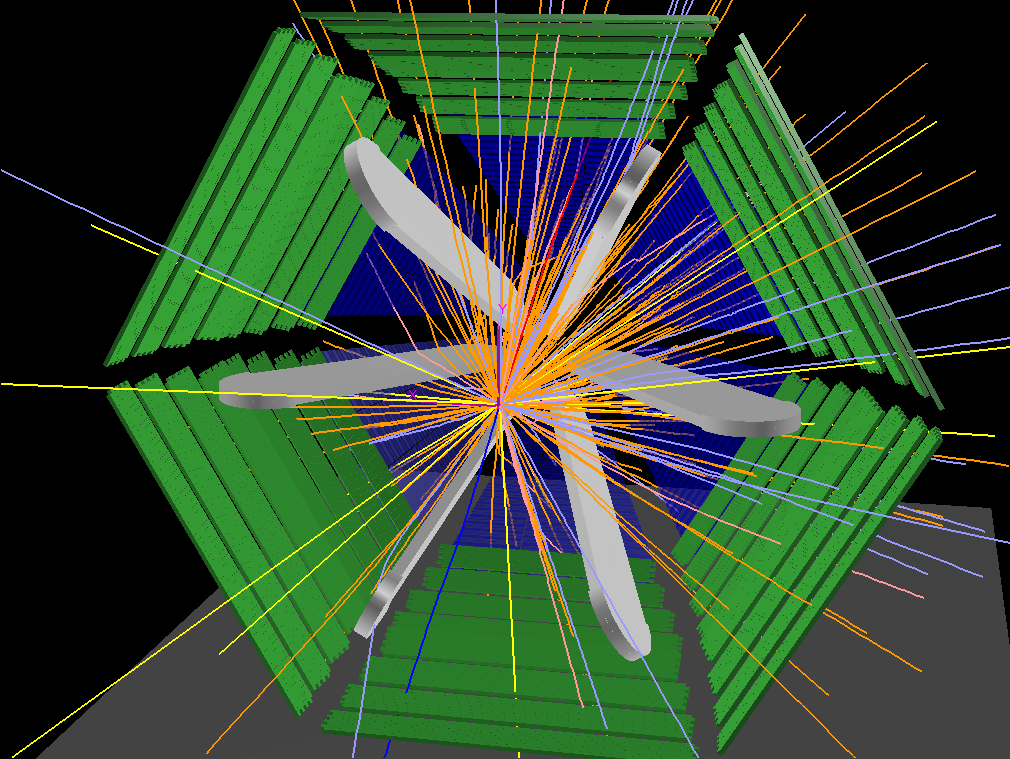
\includegraphics[width=0.8\linewidth,clip=true]{pics/eventdisplay/hades_au17au_sim_geant_iso_dark.png}
\caption[Eventdisplay for HGeant tracks]{Eventdisplay for HGeant tracks.} \label{eventdisplay_geant}
\end{center}
\end{figure}

\begin{figure}[\htb]
\begin{center}
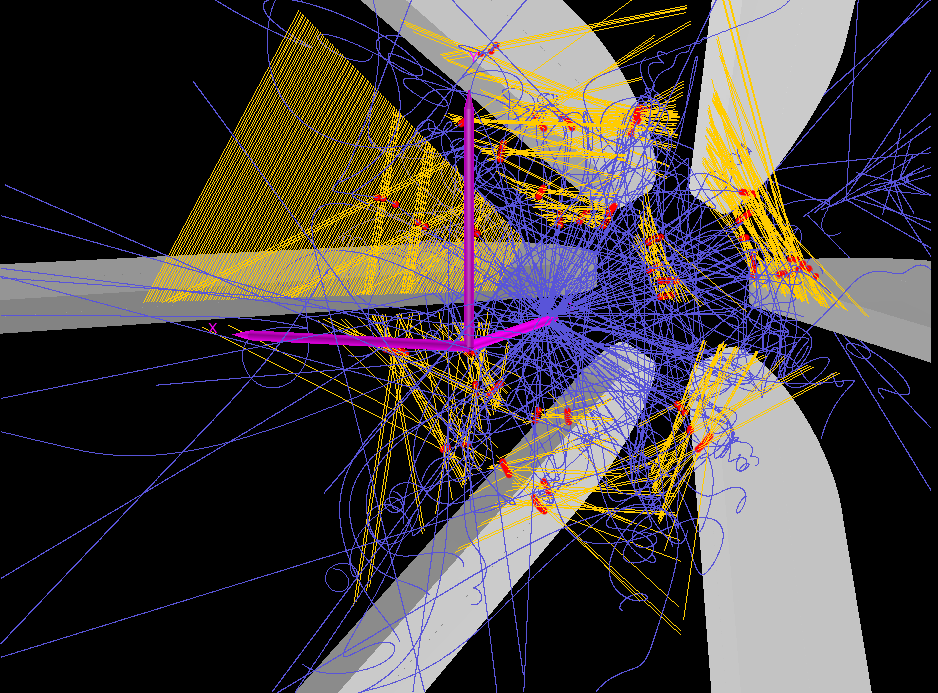
\includegraphics[width=0.8\linewidth,clip=true]{pics/eventdisplay/evt51_deltaelectrons_wires.png}
\caption[Eventdisplay for HGeant tracks]{Eventdisplay for HGeant tracks. Delta electron close
to the magnet coils.} \label{eventdisplay_deltas_geant}
\end{center}
\end{figure}



The Hades evcent 3D display is build on pure ROOT technology.
It makes use out of the ROOT build in \verb+TEve+ display and 
\verb+TGeoManager+.
It uses openGL and therefore can be used on local and remote 
(via X11) place but not via VNC (since VNC does not support openGL).

The HADES eventdisplay is provided by macros located in
the HYDRA2 module eventdisplay and the compiled library
\verb+libEventDisplay.so+ created during the standard 
make of HYDRA2.

The display uses \verb+TGeoManager+ to display the HADES detector
geometry. A ROOT file containing +TGeoManager+ can be created
by a macro. As input for the display the ROOT file is used.
The library provides objects to display hits of the different
detectors and and automtic filling of this objects from
the standard analysis objects.


\section{HOWTO setup}

To run the prepared example for central Au+Au@1.5AGeV collisions: 
\begin{lstlisting} [language=bash]

 Copy all macros HYDRA/eventdisplay/*.C 
 to your local dir. You may need
 to edit them according to your needs.

 To start in ROOT session: .x eventDisplay.C+
\end{lstlisting}

A short verview over the functionanlity of the macros and
if the user need to edit them is given below:

\begin{lstlisting}
  eventDisplay.C  : USER ACTION : setup the TGeomManager root file
  loadHadesGeom.C : NO USER ACTION required here.
  make_GUI.C      : NO USER ACTION required here.

  createHades.C   : USER ACTION required here.
                    creates HADES including detectors,
                    parameter and data sources. Setup and
                    taskslists can be changed here.
                    Basically a DST macro. This example
                    is done for Au+Au@1.5AGev simulation

  nextEvent.C     : USER ACTION required here.
                    loads one HADES event into memory. Copy
                    of hits and tracks to Eve objects is
                    done here. The user can select / group
                    and change property of the displayed
                    objects. The parts where the user should
                    edit the macro are markerd
                    "######## USER ACTION #####"
\end{lstlisting}


\section{The macros}

This section decribes the functionality of the different
macros and how the are linked together in more depths.


\verb+loadHadesGeom.C+
Reads HADES geometry from root file containing \verb+TGeoManager+.
All volumes are set invisible by default and only some
selected volumes are set visible again with the desired
color and transparency. If the \verb+TEveManager+ does not
exist it will be created. The Geometry will be added
to the global scene (persistent). The pointer to the used
\verb+TGeoVolumes+ and \verb+TGeoNodes+ are stored in 
\verb+HEDColorDef+. This
object is used by the GUI for changing the properties later.
Compiled on load time. Coordinate transformations for the
RICH pad plane and mirror are stored too.

\verb+make_GUI.C+
Creates the GUI for Display setup in \verb+TEve+. Connect
"next Event" button to 
\newline
\verb+HEDEvtNavHandler+ defined in
\verb+nextEvent.C+. Compiled on load time.

\verb+nextEvent.C+
loads a new event into memory.
It performs a call to Hades event loop. After
running the event loop the full event is available
in memory. The different detector hits can be selected
by the user, tranformed and added to the event scene of
\verb+TEve+. All objects of the previous event scene will be
destroyed.
The class \verb+HEDEvtNavHandler+ is defined here. It
is event handler to connected to the GUI.
This Class provides the \verb+selectEvent()+ function connected
to the "next Event" button. The function then calls
\verb+nextEventLoop()+ or \verb+nextEvent()+ depending if 
the the loop box is checked.
\verb+HEDEvtNavHandler+ holds the user defined 
\verb+TEveElementLists+ which are inserted in the Event 
Scene of \verb+TEveManager+. The user has to clean and 
fill this lists inside \verb+nextEvent()+.
The lists appear in "Eve" tab of the GUI in the browser
"Scenes/Event scene". The parts where the user should
edit the macro are markerd \verb+"######## USER ACTION #####"+
Compiled on load time.

\section{Available graphic objects}

The available graphic objects are defined
\verb+libEventDisplay.so+, (\verb+hedhitobjects.h+,
\newline
\verb+hedhelpers.h+)

The Eventdisplay uses LAB coordinates with x,y.z units 
in mm. Hence all hits objects from the analysis have to be
transformed to LAB and cm (TEve units). Functions used 
for coodinate transformations are located in \verb+HEDTransform+. 
\verb+HEDMdcWireManager+ will do the count statistics for 
the MDC wires. \verb+HEDGroup+ and \verb+HEDGroup2D+ 
provide some help to group
\verb+TEveElementLists+ in 1 or 2 dim arrays. This is useful
to group graphic object like sector or sector/module.
expample:
\begin{lstlisting}
  HEDGroup* sectors  = new HEDGroup("sectors","sectors",6,"Sector");
  // will create 1 main list containing 6 lists one for each sector.
  sectors->AddElement(Int_t sector,TEveElement* el)
  // will add an object to the list of the sector. The elements
  //can be TEveElementLists allowing to create complex structures.
\end{lstlisting}

The following graphical objects to display Detector hits
and tracks are available and work for REAL/SIM data:

\begin{lstlisting}
 HEDVertex          : public TEvePointSet (no input needed)
 HEDSegment         : public TEveLine     ==> HEDSegment(HMdcSegSim*)
 HEDMdcWire         : public TEveLine     ==> HEDMdcWire(HMdcCal1Sim*)
 HEDRichHit         : public TEveLine     ==> HEDRichHit(HRichHitSim*)
 HEDRichHitPadPlane : public TEvePointSet ==> HEDRichHitPadPlane(HRichHitSim*)
                      // RICH hit at pad plane
 HEDRichRing        : public TEvePointSet ==> HEDRichRing(HRichHitSim*)       
                      // RICH ring at pad plane
 HEDRichPadPlane    : public TEveQuadSet  ==> HEDRichPadPlane(Int_t sector)   
                      // RICH pad plane + fired pads
 HEDRichCompound    : public TEveCompound ==> HEDRichCompound(HRichHitSim*)   
                      // RICH hit at pad plane + ring + mirror hit
 HEDTofHit          : public TEvePointSet ==> HEDTofHit(HTofHitSim*)
 HEDTofCluster      : public TEvePointSet ==> HEDTofCluster(HTofClusterSim*)
 HEDRpcCluster      : public TEvePointSet ==> HEDRpcCluster(HRpcClusterSim*)
 HEDShowerHit       : public TEvePointSet ==> HEDShowerHit(HShowerHitSim*)

 HEDParticleCand : public TEveCompound ==> HEDParticleCand(HParticleCandSim*)
    consist out of all detector hits contributing to
    the candidate. The object provives functions
    to change the graphical representation/

    void SetLineColor  (Color_t val)
    void SetLineStyle  (Style_t val)
    void SetLineWidth  (Style_t val)
    void SetMarkerColor(Color_t val)
    void SetMarkerStyle(Style_t val)
    void SetMarkerSize (Size_t val)
    void SetRnrLine    (Bool_t val)  // kTRUE: line  will be shown
    void SetRnrPoints  (Bool_t val)  // kTRUE: points will be shown

 HGEANT OBJECTS
 TEveTrack* track = HEDTransform::createKineParticle(kine,simTrackList->GetPropagator());
                  : HEDField keeps the HADES filed map. The Runge Kutta propagator
                  : of Eve is used to propagate the track trough the detector.
 HEDRichGeantPadPlane : to draw GEANT hits on the RICH PADplane
 HEDRichGeantMirror   : to draw GEANT Mirror hits
\end{lstlisting}


\begin{figure}[\htb]
\begin{center}
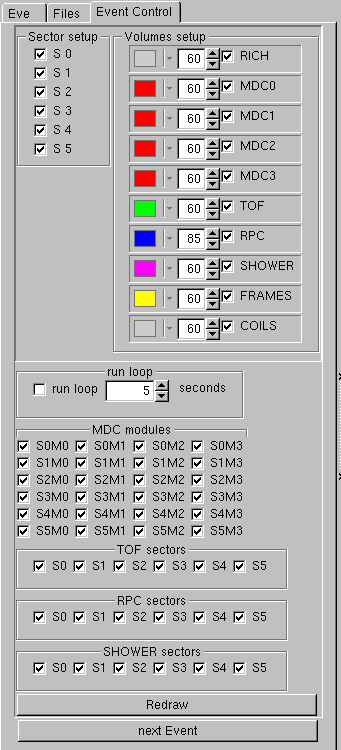
\includegraphics[width=0.4\linewidth,clip=true]{pics/eventdisplay/eventControl.png}
\caption[Eventdisplay event control]{Event control tab of the Eventdisplay. Colors , transparency 
and visability of the detectors can be set here. After the change the "Redraw" button has 
to be pressed.} \label{eventdisplay_control}
\end{center}
\end{figure}

\begin{figure}[\htb]
\begin{center}
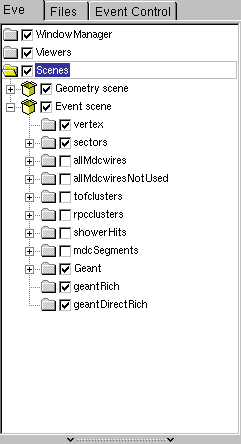
\includegraphics[width=0.4\linewidth,clip=true]{pics/eventdisplay/eveTree.png}
\caption[Eventdisplay eve tab]{Eve tab of the Eventdisplay. All graphical objects in the scene 
are eachable via this tab. The "Geometry Scene" contains the the geometrial Volumes
of the Detector. The "Event Scene" owns all objects created by the user in the "nextEvent()" 
function.} \label{eventdisplay_tree}
\end{center}
\end{figure}

\begin{figure}[\htb]
\begin{center}
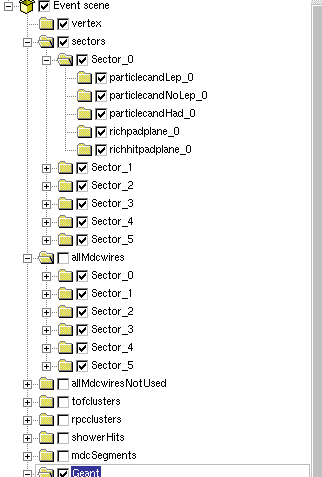
\includegraphics[width=0.4\linewidth,clip=true]{pics/eventdisplay/treeReco.png}
\caption[Eventdisplay eve tab - reco objects]{Eve tab of the Eventdisplay. 
Shown are the reconstructed objects. The objects are ordered by groups of the 
sector of the detector.} \label{eventdisplay_tree_reco}
\end{center}
\end{figure}

\begin{figure}[\htb]
\begin{center}
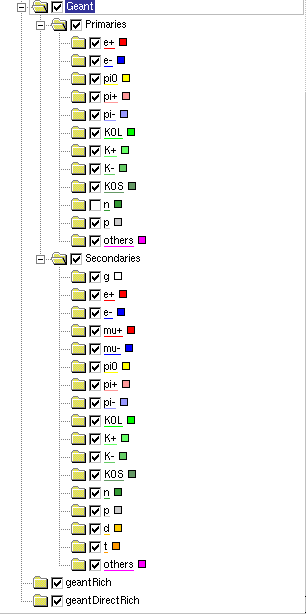
\includegraphics[width=0.4\linewidth,clip=true]{pics/eventdisplay/treeGeant.png}
\caption[Eventdisplay eve tab - HGeant objects]{Eve tab of the Eventdisplay. Shown are the HGeant 
objects. Primary and secondary particles are sorted into diffent lists. Each of the
lists keeps a list for each particle species. The particle trajectories are calulated using
the HADES magnetic field map and are propagated by a Runge-kutta algorithm through the 
detector.} \label{eventdisplay_tree_geant}
\end{center}
\end{figure}




 \clearpage
 \chapter{Event embedding}\label{Chapter_embedding}

\section{Overview}

Embedding of simulated tracks into real data events is a common 
technique to find out about the reconstruction efficiency of your 
code under realistic conditions. Realistic in the sense that 
background to the simulated tracks is as reaslitic as possible 
as the real events contain any contribution from materials which 
maybe are missing in your simulation and also you get a perfect 
noise simulation of your detector for free.

\section{Needed HYDRA and HGEANT versions}

To get the embedding running up to the PID and PAIR level and to take 
into account the event vertex properly you have to use HYDRA v8.15 or later, 
HGeant v8.15 and PLUTO (later than Dec 12 2007). Read the entries under 
open issues.


\section{How does the HADES track embedding work?}

To reach the goal of merging real and simulated tracks into one event one 
has to play some tricks.

\begin{itemize}
    \item The analysis macro will more or less look like a normal DST 
    macro for real data. The detector tasksets will be configurated 
    for real data and added to the hades taskset real. All unpackers 
    have to be configured and running.
    \item The data will filled in the simulation type to allow the 
    transportation of the \verb+HGeant+ informations
    \item Hades has to be switched to global embedding mode (see next paragraph)
    \item To data inputs have to be provided (see next paragraph)
         \begin {enumerate}
          \item hld file
          \item root file with simulated events
         \end{enumerate}
    \item In the simulation input should be always more events available 
    than in hld input. In the other case the simulation events will be 
    reused multiple times as the ROOT source rewinds when reaching the 
    file end. The sim source will not read a new event if the \verb+kSkipEvent+ 
    flag is emmitted by a task. Thus the second input has to provide 
    as many events as realy analyzed and not skipped events.
    \item The detector taskssets are reconfigurated automatically to allow 
    the embedding. Unpackers/calibraters have to fill the sim catgeories 
    before the digitizers run. The digitizers will perform all neccessary 
    actions to merge real and simulated detector hits in a realistic way. 
    Timing detectors will sort hits by time to find out which hit would 
    have created the hit. Charge detectors add the charge of multiple hits etc.
    \item Detector hits resulting from real data will contain a 
    negative tracknumber (-500 at the moment). The track number for real 
    hits can be retrieved via \verb+gHades->getEmbeddingRealTrackId()+
    \item All higher analysis tasks following the detector classes have 
    to run in simulation mode if the \verb+HGeant+ information is used. This 
    tasks should be able to handle negative \verb+HGeant+ track numbers 
    for the real detector hits.
    \item All parameter containers needed by the digitizers have to be 
    validated in ORCALE for the real data to allow the parallel use of 
    sim and real analysis.
    \item The geometry used in simulation should be the same as in real 
    data analysis. In embedding mode the geometry for the real data will 
    be used thus introducing a bias to the simulated events if both 
    geometries are not identical. This holds also for the target position.
\end{itemize}

\section{What do I need to change in my macro?}

There are 2 major things which have to set in the macro:

  (1) You have to tell Hades that you want to embedd simulated 
  tracks in real events:

\begin{lstlisting}
  //--------------------------------------------------------
  // Switch Hades to embedding mode
  // the gHades->getEmbeddingMode() flag will be analyzed
  // by all tasksets and the configuration will be switched
  // to the needs of embedding
  Hades* myHades=new Hades;
  gHades->setEmbeddingMode(1);
  //--------------------------------------------------------
\end{lstlisting}

  (2) You have to configure the second ROOT source to read your 
  simulated events:

\begin{lstlisting}
  HldFileSource *source=new HldFileSource;
  source->setDirectory("/my_dir_for_hld_files/");
  source->addFile("myhld.hld",refRun);
  myHades->setDataSource(source);


  //--------------------------------------------------------
  // root source for sim (GEANT output) (second data source)
  HRootSource *sourceSim=new HRootSource(kTRUE,kTRUE);
  sourceSim->setDirectory("/my_dir_for_sim_root_files/");
  sourceSim->addFile("mysimfile.root");
  gHades->setSecondDataSource(sourceSim);
  //--------------------------------------------------------
\end{lstlisting}

The settings above are automatically handled if one uses the 
\verb+HDstEmbedding+ class from the \verb+libDst.so+.

\section{Needed ingredients}

All parameters for the digitizers have to be validated for the real runs:
\begin{itemize}
    \item MDC : \verb+HMdcCellEff+ (cell effciency according to HV settings, 
    has to be in sync with 
    \newline
    \verb+HMdcCal2ParSim+), \verb+HMdcWireStat+ 
    (list of broken wires/missing Mbos), \verb+HMdcDigitPar+ (layer 
    efficiencies adjustments), \verb+HMdcSetup+ (adjustment of digitizer 
    parameters)
    \item RICH : \verb+HRichDigitisationPar+
    \item TOF : \verb+HTofCalPar+ context "TofCalProductionSimEmbedding" 
    (validated open end, needs only to be changed if somebody decides 
    to change something in simulation)
    \item TOFINO: \verb+HTofinoDigitPar+ (validated open end needs to 
    changed only if somebody wants to change something in simulation)
    \item SHOWER: \verb+HShowerDigiDetPar+ and maybe \verb+HShowerSimulPar+ 
    (not yet used in my version as I do not agree on the implemantation)
    \item Geometry including target poistion: Has to be identical in 
    simulation and real analysis to consistent in embedding

\end{itemize}

\section{Open issues}

\begin{itemize}
     \item Start time reconstruction in pp data: Not yet thought carefully 
     how to do it consistently.
    \item Event class selection: Not needed for C+C but for larger systems ....
    \item TOF detector : double hit handling for high multiplicities
    \item RPC detector : to be implemented
    \item WALL detector : to be implemented
\end{itemize}         

\section{How-to take into account the event vertex}

For ananalysis which applies a vertex cut the event vertex has to be 
properly taken into account during the event embedding to estimate 
the reconstruction efficiencies.
\begin{enumerate}
    \item Write out a vertex ntuple file using \verb+HMdcVertexWriter+ 
    for the hld file which will be used for embedding. The vertex ntuple 
    contains the 3 vertex coordinates + Event seq Number. Only events are 
    taken into account where a vertex could be calculated.The task should 
    be connected last to the tasklist to make shure that only events are 
    written out which have not been skipped.
    \item The vertex ntuple is used with a PLUTO macro to generate the 
    embedded particles at the same vertex as in the real data. The PLUTO 
    ascii file (.evt) contains beside the vertex the event seq number, 
    which will be stored in \verb+HGeantKine::userVal+. After running 
    \verb+HGeant+ the output root file contains the same vertices as the 
    real data. The transported event seq number is used to synchronize 
    the embedded events with the real events.
    \item In embedding mode the \verb+HMdcVertexfind+ works different 
    from sim or real. Several settings can be done via the static functons
     \begin{lstlisting}
     // setup the vertexfinder for embedding
     HMdcVertexFind::setRejectEmbeddedTracks(kTRUE);   // (default: kTRUE)  reject embedded tracks from vertex calculation (needed if no event seq is used)
     HMdcVertexFind::setUseEventSeqNumber   (kTRUE);   // (default: kTRUE)  use the event seq number stored in HGeantKine
     HMdcVertexFind::setSkipNoVertex        (kFALSE);  // (default: kFALSE) kTRUE: skip events where no vertex could be calculated
     \end{lstlisting}
     The event seq number will be used to match the events in default mode. 
     The vertex will not be calculated instead it will be taken from \verb+HGeant+ 
     (primary particle) This procedure ensures to get exactly the same 
     vertex as without embedded particles.
\end{enumerate}

\section{How-to create embedded particles with PLUTO using a vertex ntuple}

The following example program reads an vertex ntuple file and creates a 
white spectrum of positrons with PLUTO. The .evt file will contain particles 
comming from the same vertex as the real data which have been used to 
create the vertex file.This output can be read by \verb+HGeant+. Needs 
HYDRA v8.15 or later, HGeant v8.15 or later and PLUTO (> Dec 12 2007). 
Copy to your local dir.

\begin{itemize}
    \item \verb+setenv_pluto.sh+: setup environment for ROOT + PLUTO

    \item \verb+run_pluto_embedded.make+: Makefile for 
    \verb+run-pluto-embedded program+

    \item \verb+run_pluto_embedded.cc+: \verb+run-pluto-embedded+ program

    \item \verb+pluto_embedded.cfg+: configuration file for 
    \verb+run-pluto-embedded+ program
\end{itemize}

To compile the program setup yout hydra like

\begin{lstlisting}
  . ./setenv_pluto.sh

  make -f run_pluto_embedded.make clean build install

  ./run_pluto_embedded --cfg-file pluto_embedded.cfg
\end{lstlisting}



\section{How-to setup HGEANT ini.dat for reading PLUTO with vertex coordinates}

Write your \verb+HGeant+ init.dat file as usually. Your configuration should not 
contain the \verb+HGeant+ keywords \verb+JVER+ and \verb+BEAM+. The vertices of the 
particles are used from the .evt input file of PLUTO. \verb+HGeant+ recognizes the 
format by analyzing the header flags of the event. Make shure that the used 
geomtery matches the one from real data.

\section{Full working embedding chain example}

On the page linked here you will find a full working chain of macros 
and scripts used for the efficiency calculation of APR06. This set 
includes the production of vertex.root files, PLUTO .evt files, \verb+HGeant+ 
processing and embedded DST production. Scripts for running batch 
are provide too. 

\section{Data flow}

In the following the data flow of the different detector systems will be displayed 
to explain on which entry levels the real data hits are merged with the simulated 
ones. As usual all detectors behave a bit different according to their special 
needs and the programmers will to stick to standards. The special actions will 
be decribed in the detector sections below.

\subsection{RICH}

In embedding mode the internal noise simulation of the \verb+HRichDigitizer+ will be 
switched of no matter if or not the rich taskset has been configured for using 
noise simulation. The noise in that sense will be created by the real events 
itself. Note that the real hits can be identified by the triplet 
tracknumber/flag/energy as shown below in the table. 

\begin{lstlisting}
 realID=gHades->getEmbeddingRealTrackId()

                        track Number      Flag     energy
  Cheren. Phot.            #               0        #
  Feedback Phot.          -5               0        0
  Direct Hits              #               1        0
  Noise Hits               0               0        0  
  REAL Hits (embedding)    realID          0        0
---------------------------------------------------------


   ----------------                            ------------
  |  HRichUnpacker |                          | HGeantRich |
  |(embedding mode)| \                         ------------
  |                |  \                             ||
   ----------------    \                            || input 
                        \                           \/
                   -------------  read real     ----------------
                  | HRichCalSim | ---------->  |                |
                   -------------  <---------   |                |
                                               | HRichDigitizer |
                   -------------               |                |
                  | HRichTrack  | <---------   |                |
                   -------------                ----------------
                                  write output
\end{lstlisting}

\subsection{MDC}

For the embedding of the MDC data the embedding flag set in \verb+HMdcSetup+ 
will be overridden by the global Hades embedding mode if detected. For a 
realistic embedding the cuts on drift times are shifted from the \verb+HMdcCalibrater1+ 
to the clusterfinder. This allows the embedding before the cuts are applied.

\begin{lstlisting}
   --------------                               -----------
  | HMdcUnpacker |                             | HGeantMdc |
   --------------                               -----------
         |                                          ||
   ----------------                                 || input 
  |HMdcCalibrater1 |                                \/
   ----------------      -------------   read    ---------------
                   |--->| HMdcCal1Sim | ------> | HMdcDigitizer |
                         -------------  <-----  |               |
                                         write   ---------------
                                         
\end{lstlisting}

\subsection{TOF}

As the tof calibration is done for left and right rod hit together the embedding 
is shifted to the hit level. In that case the digitizer will write a non-persistent 
\verb+catTofRawTmp+ category. The \verb+HTofHitF+ task will create a non-persistent 
\verb+HTofHitTmp+ category for simulated tracks and in a second step merge the 
simulated and real hits in the final output category. The calibration for real 
and simulated hits is fully consistent. In the case a rod was hit by a real and 
a simulated track, the simulated hit will be propagated. In future the merging 
should be done in a realistic fashion. In C+C at 2AGeV this cases are at the order 
of 0.3\%. In case of a pure simulation none of those tmp categories will be used 
and the data flow will look like in real data.
\begin{lstlisting}
                                      ------------                      
                                     | HGeantTof  |                     
                                      ------------                      
                                           |                            
   ----------------------           -----------------                   
  |     HTofUnpacker     |         |  HTofDigitizer  |                  
  |   (embedding mode)   |      -- |                 |                  
  |                      |     /   ------------------                   
   ----------------------     /             |                           
              |              /       ----------------                   
         -------------      /       |  HTofRawSimTmp |                  
        | HTofRawSim  |----         | non persistent | (embedding mode, 
         -------------               ----------------   sim data)       
  sim (sim mode)      \              /                                  
  or real (embedding)  \            /                                   
                       -----------------                                
                      |  HTofHitFSim    |                               
                       -----------------                                
                       /       |                                        
                      /  ----------------                               
                     /  | HTofHitSimTmp  | (embedding mode              
                    /   | non persistent |  sim data )                  
                   /     ----------------                               
                  /     /                                               
                 /     /                                                
         -------------                                                  
        | HTofHitSim  | sim (sim mode) or                               
         -------------  sim and real data                               
                        (embedding)                                     
                                                                        
                                                                        
                                                                        
  In the case of TRACK EMBEDDING of simulated tracks into
  experimental data the real data are written by the HTofUnpacker into
  HTofRawSim category. In embedding mode the digitizer will write his
  output to HTofRawSimTmp to merge real and sim data on hit level
  (keep calibrations constistent).
\end{lstlisting}

\subsection{SHOWER}

Thanks to the complicated data structure of the shower analysis the embedding 
actions had to be split to \verb+HShowerPadDigitizer+ and \verb+HShowerCopy+.

\begin{lstlisting}
   ------------------
  | HShowerUnpacker  |                                                                   
  |(embedding mode)  | \                                                                 
  |                  |  \     --------------                                             
   ------------------   |    | HGeantShower |                                            
                        |     --------------\                                            
                        |                    \                                           
                        |     --------------  \---------> ----------------------          
                        |    | HGeantWire   |  <-------- |  HShowerHitDigitizer |         
                        |     ---------------\            ----------------------          
                        |                     \                                      
            -------------     ---------------  \------->  ----------------------         
        -- | HShowerRaw  |   | HShowerRawMatr|   <------ |  HShowerPadDigitizer |        
       |    -------------     ---------------\           |( create track objects|        
       |                                      \          |  for real tracks in  |        
   ----------------------     --------------   \         |  embedding mode too) |        
  |   HShowerCalibrater  |   | HShowerTrack |  <--------- ----------------------         
  |   (embedding mode)   |    --------------\    \                                        
   ----------------------                    \    \       ----------------------         
       |                      --------------  \    ----> |   HShowerCopy        |        
        -------------------> | HShowerCal   |  \<------- |(add charge of real   |        
                              --------------\   \        | hit in embedding too)|        
                                             \   \        ----------------------         
                              --------------  ----\---->  ----------------------         
                             | HShowerHitHdr|   <--\---- |  HShowerHitFinder    |        
                              --------------        \     ----------------------         
                              --------------         \      |                             
                             | HShowerPID   |   <-----\-----|                             
                              --------------           \    |                             
                              --------------            \   |                             
                             | HShowerHit   |   <--------\--|                             
                              -------------- <            \                               
                                              \            \                              
                                               \--------->-----------------------        
                                                         | HShowerHitTrackMatcher|       
                                                          -----------------------        

  In the case of TRACK EMBEDDING of simulated tracks into
  experimental data the real data are written by the HShowerUnpacker into
  HShowerRaw category. The real hits are taken into
  account by the digitizer (adding of charges). The embedding mode is recognized
  automatically by analyzing the
  gHades->getEmbeddingMode() flag.
            Mode ==0 means no embedding
                 ==1 realistic embedding (first real or sim hit makes the game)
                 ==2 keep GEANT tracks   (as 1, but GEANT track numbers will always
                     win against real data. besides the tracknumber the output will
                     be the same as in 1)

\end{lstlisting}



 \clearpage
 \chapter{HADES online monitor}

\section{How-to setup and run server/client}

%-----------------------------------------------------
\begin{enumerate}
   \item  set environment : \verb+. /misc/kempter/svn/hydraTrans/defalls.sh+
   \item  build sever/client:
\begin{lstlisting}
   
cd /misc/kempter/svn/hydraTrans/online/server/
make clean build install
cd /misc/kempter/svn/hydraTrans/online/client/
make clean build install
make clean build install
\end{lstlisting}
   \item  copy config files: 
   \newline
   \verb+cp 	hydraTrans/online/client/ClientConfig.xml .+
   \item  setup  \verb+ClientConfig.xml+ for needed hists (if needed)
   \newline
   setup  \verb+analysisParams.txt+ to define parameter input , file input etc
   \item start server
 \begin{lstlisting}
 hadesonlineserver.exe name hostname port ""
 hadesonlineserver.exe OnlineMon lxg0453.gsi.de 9876 ""
 \end{lstlisting}
 \item	start client
 \begin{lstlisting}
 ./hadesonlineclient.exe  ClientConfig.xml
 ./hadesonlineclient.exe  hostname port stop   ==> stop server
 ./hadesonlineclient.exe  hostname port list   ==> print available histograms on the server
 \end{lstlisting}
\end{enumerate}
%-----------------------------------------------------


\section{How-to add/change histograms to monitoring}


\begin{enumerate}
 \item	each detector has its own monitor. 
 in online/server you find different macros:
 \begin{enumerate}
    \item \verb+hadesonlineserver.cc ==>+ main program
    \item \verb+createHades.C        ==>+ setup your server program
    \item \verb+Detectorname.C       ==>+ monitoring the detector
  \end{enumerate}
  This file contains
  \verb+createHistsDetectorname()+ 
  add hists to the histpool and a local map which is
  used to access the histograms by name
  \verb+fillHistsDetectorname()+ 
  access the histograms by name to fill them (the function
  will be called once per event)
  both functions are called from \verb+hadesonlineserver.cc+.
  \verb+hadesonlineserver.cc+ has to be recompiled and restarted
  after changes.

 \item	After the histograms are added and the fill routine is
      	defined the histogram has to be added to the Monitor GUI.
       	Simply add the histogram \verb+online/client/ClientConfig.xml+
      	New detectors can be added on the fly. The monitor client
       	does not need to be recompiled, it creates the GUI dynamically
       	by parsing the xml file. Changes on the client side needs
       	no restart of the server as long as no new histograms have
       	been defined.
\end{enumerate}

\section{Available monitoring histograms and how to use them}

\begin{enumerate}
  \item  All histogram types are derived from \verb+HOnlineMonHistAddon+.
\begin{lstlisting}         
HOnlineMonHist	   : 1-Dim Histogram
HOnlineMonHist2	   : 2-Dim Histogram
HOnlineTrendHist   : 1-Dim Trend Histgram
                     (new values added on
                     the left side of the histogram, 
                     old values moved to the right)
                
HOnlineHistArray   : 1/2-Dim Array of 1-Dim Histograms
HOnlineHistArray2  : 1/2-Dim Array of 2-Dim Histograms
HOnlineTrendArray  : 1/2-Dim Array of Trend Histograms
\end{lstlisting}         
       
  \item All histograms are created by a definition String:
In \verb+Detector.C+ in 
\newline
\verb+createHistsDetectorname.C+ :
                
\begin{lstlisting}         
Text_t* hists[] = 
{
 "FORMAT#array TYPE#1F NAME#hMdctime1Cal1 TITLE#Mdc_timeCal1 ACTIVE#1 RESET#1 REFRESH#5000 BIN#800:-100:700:0:0:0 SIZE#1:2 AXIS#time_[channel]:counts:no DIR#no OPT#no STATS#0 LOG#0:1:0 GRID#1:1 LINE#1:0 FILL#0:0 MARKER#0:0:0 RANGE#-99:-99"
 ,"FORMAT#mon TYPE#1F NAME#hMdctime1Cal1MeanTrendtemp TITLE#time1Cal1MeanTrendtemp ACTIVE#1 RESET#1 REFRESH#5000  BIN#1200:0:1200:0:0:0 SIZE#0:0 AXIS#no:no:no DIR#no OPT#no STATS#0 LOG#0:0:0 GRID#0:0 LINE#0:0 FILL#0:0 MARKER#0:0:0 RANGE#-99:-99"
 ,"FORMAT#mon TYPE#2F NAME#hMdccal1hits TITLE#Mdc_hcal1hits ACTIVE#1 RESET#1 REFRESH#5000 BIN#8:0:4:12:0:6 SIZE#0:0 AXIS#module:sector:no DIR#no OPT#lego2 STATS#0 LOG#0:0:0 GRID#1:1 LINE#0:0 FILL#0:0 MARKER#0:0:0 RANGE#-99:-99"
 ,"FORMAT#trendarray TYPE#1F NAME#hMdccal1hitstrend TITLE#Mdc_hcal1hits_trend ACTIVE#1 RESET#0 REFRESH#500 BIN#50:0:50:0:0:0 SIZE#6:4 AXIS#trend:multiplicity:no DIR#no OPT#p STATS#0 LOG#0:0:0 GRID#0:1 LINE#0:0 FILL#0:0 MARKER#1:20:0.5 RANGE#-99:-99"
 ,"FORMAT#mon TYPE#2F NAME#hMdcrawRoc_Subev TITLE#Mdc_Raw_Roc_SubEvent_Size ACTIVE#1 RESET#0 REFRESH#5000 BIN#120:0:24:40:0:160 SIZE#0:0 AXIS#no:sub_evt_size:counts DIR#no OPT#COLZ STATS#0 LOG#0:0:0 GRID#1:1 LINE#0:0 FILL#0:0 MARKER#0:0:0 RANGE#-99:-99"
 ,"FORMAT#array TYPE#2F NAME#hMdcmbotdcCalib TITLE#Mdc_mbo_tdc_calib ACTIVE#1 RESET#1 REFRESH#5000 BIN#16:0:16:12:0:12 SIZE#6:4 AXIS#mbo:tdc:no DIR#no OPT#colz STATS#0 LOG#0:0:0 GRID#1:1 LINE#0:0 FILL#0:0 MARKER#0:0:0 RANGE#-99:-99"
};
\end{lstlisting}         

  \begin{enumerate}
    \item The names of the histograms must be unique.
    To avoid overlap with other detectors use
    \verb+hDetectorname+..... 
    They are used to retrieve the histograms by the
    clients and inside the macros.
    \item FLAGS inside the definition:
\begin{lstlisting}         
FORMAT:         mon             ==> HOnlineMonHist
                array           ==> HOnlineHistArray / OnlineHistArray2
                trendarry       ==> HOnlineTrendArray
TYPE:           1F / 2F         ==> 1/2 Dim Histograms
NAME:                           ==> name of Histogram
ACTIVE:         0/1             ==> Create Histogram
RESET:          0/1             ==> Should the Histogram be refreshed if the 
                                    Refresh count is reached ?
REFRESH:                        ==> N events before reset 
BIN:   nBinsX:xMin:xMax:nBinsY:yMin:yMax
                                ==> definition for Histogram (leave y values 0 for 1 Dim)
SIZE:      nx:ny                ==> 2-Dim array definition for FORMAT 
                                    array/trendarray
           1:n         1-Dim
           0:0         no array
\end{lstlisting}         
    \item \verb+mapHolder::createHists(Int_t size,hists,histpool)+;
     will create the Histrograms according to the definition and add them to the 
     pool of Histograms on the server and the 
     \newline
     \verb+std::map <TString, HOnlineMonHistAddon*> detnameMap+
     defined inside the macro.
    \item The histograms can be accessed with \verb+get("histogramname")+
    inside the macro. In case the name is not contained in 
    \item Fill histograms : From any histogram type you can retrieve the
    pointer to the standard ROOT histograms by
\begin{lstlisting}         
                        
get("histogramname") -> getP()     // 1-Dim
get("histogramname") -> getP(0,i)  // 1-Dim array
get("histogramname") -> getP(i,j)  // 2-Dim array
                        
For trend histograms / array trend histograms
use special fill() function.
 
get("histogramname") -> fill(val)     // 1-Dim
get("histogramname") -> fill(0,i,val) // 1-Dim array
get("histogramname") -> fill(i,j,val) // 2-Dim array
\end{lstlisting}         
                      
    \item How-to USE trend histograms: trend histgrams are usually filled 
    with some variables which are obtained as avarage over several events 
    (like avarage count rate, mean values, rms etc). The strategy is to 
    fill a temporary histogram to collect the values over the events and 
    if the refreshrate of the trend histogram is reached get the needed 
    values from the temp histograms and fill them to the trend. It could 
    look like:
\begin{lstlisting}         
                        
 // loop over data for each event
 // inside fillHistsDetectorname(evtCt)
        
 HCategory* mdcRawCat = gHades->getCurrentEvent()->getCategory(catMdcRaw);
 HMdcRaw* raw;
 for(Int_t i = 0; i < mdcRawCat->getEntries(); i ++) {                  	
     raw = (HMdcRaw*)mdcRawCat->getObject(i);
     if(raw) {
              get("histtrendtemp")->getP()->Fill(raw->getTime(1));
     }
 }
 // end loop
                        
 //---------------------------------------
 // now fill trend hist
 if(get("histtrend") && get("histtrendtemp") && // both hists exists
    evtCt%get("histtrend")->getRefreshRate() ==0 && evtCt > 0){ 
    // reached refresh
    get("histtrend")->fill(get("histtrendtemp")->getP()->GetMean());
    get("histtrendtemp")->getP()->Reset(); // now rest the tem hist
 }
 //---------------------------------------
\end{lstlisting}         
  \end{enumerate}                 
\end{enumerate}                 
                        
                        
\section{How-to add histograms to the client GUI} 
        
\begin{enumerate}        
\item The configuration of the Client is done via \verb+online/clien/ClientConfig.xml+
\item The Client does not need to be recompiled
\item Each detector GUI is created on the fly by parsing 
the xml file.It might look like:
          	
\begin{lstlisting} [language=XML]        
  // in xml file
  //---------------------------------------
  <client> 
             
    <!-- program configuration -->
    <config>
    <server>
    <host>hostname</host>     // host where the server is running
    <port>portnumber</port>   // potnumber for connection to server
    </server>
    </config>
    
    
     <!-- configuration for main window -->
     <MainWindow>
        <name>HADESMonitoring</name>
        <title>HADES Monitoring</title>
        <width>200</width>
        <height>400</height>
     </MainWindow>
             
             
     <!-- detector configuration -->
     <detector>
        <name>TOF</name>     // this name will be use inthe main panel
        <title>TOF</title>
       	<window>
          <name>TOFMon</name>
          <title>TOFMon</title>
          <tabbed>true</tabbed>  // the window will contain tabs
          <tab>
             <name>Main</name>   // first tab name
             <title>Main</title>
             <canvas>            // canvas inside tab
             	<name>Main</name>
              	<width>1000</width>  // size of canvas
              	<height>800</height>
               	<splitted>true</splitted> // create 3x2pads
               	<nx>3</nx>
               	<ny>2</ny>
              	<histogram>               
              	    <name>hdetectorname</name> //name of histogram
              	    <type>single</type>        // plot hist or allhists of array
              	    <subpad>1</subpad>         // pad number starts from 1 (0 if not splitted)
               	</histogram>
                <histogram>               
               	    <name>hdetectorname2array</name> //name of histogram
              	    <type>array:0:0</type>           //plot hist with index of array
               	    <subpad>1</subpad>               //pad number starts from 1 (0 if not splitted)
               	</histogram>
                             
              </canvas>
          </tab>
        </window>
     </detector>
  </client>
  //---------------------------------------
            
  DO NOT PUT THE // comments INTO YOUR REAL CONFIG!!
  FOR ALL POSSIBLE TAGS LOOK DOCU INSIDE XML FILE.
\end{lstlisting}         
\end{enumerate}        
       
        







 \clearpage



 %GATHER{lit_article.bib}       % For Gather Purpose Only
 %GATHER{lit_book.bib}          % For Gather Purpose Only
 %GATHER{Lit_misc.bib}          % For Gather Purpose Only

% ------------------------------------------------------------------------
 \begin{appendix}
  \chapter{Appendix macros}


  \chapter{Appendix}

 \end{appendix}

\cleardoublepage
\bibliographystyle{alpha}
\bibliography{lit_article,Lit_book,Lit_misc}
% ------------------------------------------------------------------------

\cleardoublepage

% ------------------------------------------------------------------------
\end{document}
% ------------------------------------------------------------------------
